\documentclass[11pt]{amsart}
\usepackage{amsmath,amssymb,amsthm}
\usepackage[margin=1.1in]{geometry}
\usepackage[expansion=false]{microtype}
\allowdisplaybreaks
\usepackage{enumitem}
\usepackage{array,booktabs}
\newcolumntype{R}[1]{>{\raggedright\arraybackslash}p{#1}}
\usepackage{graphicx}
\graphicspath{{../figures/}}
\usepackage[colorlinks=true,linkcolor=blue,citecolor=blue,urlcolor=blue]{hyperref}
\hypersetup{pdftitle={Sums of two squares and Heegner norms with few prime factors, IV},pdfauthor={Ruqing Chen}}
\emergencystretch=2.5em
\hbadness=1500
\raggedbottom

\newtheorem{theorem}{Theorem}[section]
\newtheorem{lemma}[theorem]{Lemma}
\newtheorem{proposition}[theorem]{Proposition}
\newtheorem{corollary}[theorem]{Corollary}
\theoremstyle{remark}
\newtheorem{remark}[theorem]{Remark}

\newcommand{\Z}{\mathbb{Z}}
\newcommand{\Q}{\mathbb{Q}}
\newcommand{\HH}{\mathbb{H}}
\newcommand{\e}{\varepsilon}
\newcommand{\dd}{\mathrm{d}}
\newcommand{\cF}{\mathcal{F}}
\DeclareMathOperator{\gen}{gen}
\DeclareMathOperator{\vol}{vol}
\DeclareMathOperator{\pr}{pr}
\DeclareMathOperator{\tr}{tr}

\title[Sums of two squares and Heegner norms, IV]{Sums of two squares and Heegner norms with few prime factors, IV:\texorpdfstring{\\}{ } the scalloped Parseval formula, the Heegner classification,\texorpdfstring{\\}{ } and Eisenstein dispersion}
\author{Ruqing Chen}
\address{GUT Geoservice Inc., Montreal, Canada}
\email{ruqing@hotmail.com}
\date{\today\ (draft)}

\begin{document}

\begin{abstract}
Parts I--III studied the cusp form $G_{m,m'}$ attached to $\theta^2(mz)\theta^2(m'z)$, whose Fourier coefficients are the remainders of the sieve for $r(n)r(N-n)$. Three results. (1)~The Petersson norm of $G$ is given \emph{exactly} by a Parseval sum over the cusps whose lower boundary is the scalloped curve $y=\sqrt{1-\{x\}^2}$ of Waibel's fundamental domain, with correlation terms $a(k)\overline{a(k+jQ)}$ at distances multiple of the width. It gives the coefficient of $\log p$ in $\|G_{1,p}\|^2=\frac1\pi(\log p)^2+B\log p+O(1)$ in closed form: $B=0.48204$ is the sum of $0.383$ from the free part of the two main cusps, $2\kappa/\pi=0.0288$ from the region between the arcs and the line $y=1$, and $0.0702$ from the coefficients $k\ge p$, a sum of exponential integrals $E_1(\pi\beta)$, $E_1(4\pi\beta)$ weighted by $r(\beta)^2$; the Siegel main term contributes nothing to $B$. (2)~For the seven odd discriminants of class number one, $D\in\{3,7,11,19,43,67,163\}$, $\Theta^{(D)}_{1,p}=\theta_D(z)\theta_D(pz)$ has the square-free level $Dp$ with four Atkin--Lehner cusps. We prove, uniformly in $D$, the Siegel main term with closed-form densities at $D$ and $p$, the Atkin--Lehner signs, the necessary condition $a_\varphi(D)=\chi_{-D}(p)$, $a_\varphi(p)=-\chi_{-D}(p)$ for a newform to occur, the Rankin--Selberg formula with the constant $C_D=w_D^2\sqrt D/(8\pi^2)$, and the asymptotic $\|G^{(D)}_{1,p}\|^2=\frac{6}{\pi(D+1)}(\log p)^2+B_D\log p+O(1)$ with $B_D$ in closed form; the leading coefficient is $2/\vol(\Gamma_0(D)\backslash\HH)$, and the corresponding lower bound holds for $D=8$ as well. (3)~For the Eisenstein integers the Fourier transform of the circle $x^2+xy+y^2\equiv a$ modulo any $c$ prime to $3$ is a classical Kloosterman sum with the hexagonal dual norm, the ramified prime $3$ takes over the role that $2$ plays for the Gaussian integers, and the obstruction to a level beyond $1/2$ is unchanged. We also correct an error of Parts~II--III: the Kloosterman sums of the dispersion form are $S(\overline{16m}N,|h|^2;m'k)$, not $S(16N,m|h|^2;m'k)$.
\end{abstract}

\maketitle
\enlargethispage{4pt}

\section{Introduction and statement of results}\label{sec:intro}

\subsection{Setting}
Parts I--III \cite{ChenI,ChenII,ChenIII} prove the level of distribution $1/2$ for the weighted sequence $r(n)r(N-n)$, $r$ the number of representations as a sum of two squares, and with it $\Omega(n(N-n))\le7$, $\max(\Omega(n),\Omega(N-n))\le5$ for every large $N\equiv2\pmod4$, through the cusp forms $G_{m,m'}\in S_2(\Gamma_0(4mm'))$ with $\theta^2(mz)\theta^2(m'z)=E_{m,m'}+G_{m,m'}$: the Fourier coefficient $a_{G_{m,m'}}(N)=T(m,m';N)-M(m,m';N)$ is the remainder of the sieve at the modulus pair $(m,m')$, and the uniform bound $|a_G(N)|\ll N^{1/2+\e}\|G\|$ (Part~I, Theorem~2.3) with $\|G_{m,m'}\|^2\asymp(\log mm')^2$ (Part~II, Theorems~1.5 and 6.14) gives the level. Part~III located the obstacles to a level beyond $1/2$ and to the pair $(7,4)$. The present part answers three questions that arose from it: how large exactly is the norm (the term $B\log p$ which Part~II, Remark~6.16, could only estimate); what happens for the other imaginary quadratic fields of class number one; and whether the Eisenstein integers, with their square-free level, change the dispersion problem.

\subsection{Results}
Let $G\in S_2(\Gamma_0(L))$. Waibel's formula \cite[(22)]{Waibel} (Part~I, Lemma~2.8) writes $\|G\|^2$ as a sum over the cusp classes of integrals of $|G|_2\varrho|^2$ over the union of the $L$ translates $t\cF$, $0\le t<L$, of the standard fundamental domain, whose lower boundary is the \emph{scalloped} curve $y=s(x)=\sqrt{1-\{x\}^2}$ ($\{x\}$ the distance to the nearest integer), not a horizontal line. Part~II bounded these integrals by the strips $y\ge1$ and $y\ge\sqrt3/2$: with $\Lambda_h$ the sum of the integrals over $y\ge h$, $\Lambda_1\le\|G\|^2\le\Lambda_{\sqrt3/2}$ (Part~II, Lemma~6.11). Parseval over the exact region gives an identity. Throughout, $S(Y)=\sum_{k\ge1}r(k)^2k^{-1}e^{-k/Y}$, $E_1(x)=\int_x^\infty e^{-t}t^{-1}\dd t$ is the exponential integral, and $\kappa=\int_{-1/2}^{1/2}\log(1-x^2)^{-1/2}\dd x=0.045231$.

\begin{theorem}[Scalloped Parseval]\label{thm:A}
For $G\in S_2(\Gamma_0(L))$ with $G|_2\varrho=\sum_{k\ge1}b_d(k)e(kz/Q_d)$ at a cusp of the class $d\mid L$ and width $Q_d$ (Section~\ref{sec:scallop}), and $\Psi_j(c)=\int_{-1/2}^{1/2}\cos(2\pi jx)e^{-c\sqrt{1-x^2}}\dd x$,
\[
\|G\|^2=\sum_{d\mid L}w_d\sum_{k\ge1}\sum_{j}b_d(k)\overline{b_d(k+jQ_d)}\,\frac{\Psi_j(c_{k,j})}{c_{k,j}},\qquad c_{k,j}=\frac{2\pi(2k+jQ_d)}{Q_d},
\]
with explicit weights $w_d$ (Proposition~\ref{prop:scallop}). For $G=G_{1,p}$ the formula, evaluated with $k\le14p$, reproduces the Rankin--Selberg estimates of Part~II where these have converged ($7.42858$ against $7.42871$ at $p=101$), lies inside the sandwich $\Lambda_1\le\|G\|^2\le\Lambda_{\sqrt3/2}$ at every $p$, and gives, over $p\ge10^4$,
\[
\|G_{1,p}\|^2=\frac1\pi(\log p)^2+B\log p+O(1),\qquad B=0.48204\ldots,
\]
where $B$ is the explicit constant of Theorem~\ref{thm:closedB}: $0.383$ is the free part $\frac1{4\pi}(S(p/4\pi)+S(p/\pi))$ of the two main cusps (Part~II, Lemma~6.3), $0.0288=2\kappa/\pi$ the arcs acting on that free part (Proposition~\ref{prop:mellin}), $0.0569$ and $0.0119$ the coefficients $k\ge p$ of the two main cusps at height $1$ and through the arcs, $\frac1\pi\sum_\beta r(\beta)^2(E_1(\pi\beta)+E_1(4\pi\beta))$ and its arc version, $0.0019$ the cusp of denominator $2$ and $-0.0005$ the correlation terms; the Siegel main term and all cross terms are $O(1)$. The fit over $10^4\le p\le4\cdot10^5$ gives $0.4817$, the local slopes at the largest primes $0.4819$ and $0.4820$.
\end{theorem}

The value $B\approx0.46$ of Part~II, Remark~6.16, was a fit to Rankin--Selberg estimates that had not converged; the fit of the exact formula gives $0.48$, and Theorem~\ref{thm:closedB} the constant itself.

Let now $D\in\{3,7,11,19,43,67,163\}$ be an odd discriminant of class number one, $\chi=\chi_{-D}$, $w_D$ the number of units, $N_D(x,y)=x^2+xy+\frac{D+1}4y^2$, $r_D(n)=w_D\sum_{d\mid n}\chi(d)$, $\theta_D=\sum r_D(n)e(nz)$ and, for a prime $p\ne D$,
\begin{gather*}
\Theta^{(D)}_{1,p}=\theta_D(z)\theta_D(pz)=E+G^{(D)}_{1,p}\in M_2(\Gamma_0(Dp)),\\
a_G(k)=T(k)-M(k)=\sum_{\alpha+p\beta=k}r_D(\alpha)r_D(\beta)-M(k).
\end{gather*}

\begin{theorem}[The odd Heegner discriminants]\label{thm:B}
\begin{enumerate}[label=\textup{(\roman*)},leftmargin=2.2em]
\item $M(k)=\frac{4\pi^2k}{Dp}\prod_\ell\beta_\ell(k)$ with the standard densities at $\ell\nmid Dp$ and, with $v=v_\ell(k)$ and $\e=-\chi_{-D}(p)$,
\[
\beta_p(k)=(1+\chi(p))-\chi(p)\Bigl(1+\frac1p\Bigr)p^{-v},\qquad \beta_D(k)=(1+\e)-\e\Bigl(1+\frac1D\Bigr)D^{-v}.
\]
\item $\Theta|_2W_p=\chi(p)\Theta$, $\Theta|_2W_D=-\chi(p)\Theta$, $\Theta|_2W_{Dp}=-\Theta$.
\item A newform $\varphi$ of level $Dp$ occurs in $G^{(D)}_{1,p}$ only if $a_\varphi(D)=\chi_{-D}(p)$ and $a_\varphi(p)=-\chi_{-D}(p)$ (root number $+1$); an oldform from level $p$ only if $a_f(p)=-\chi_{-D}(p)$; an oldform from level $D$ only if $\chi_{-D}(p)=+1$. These conditions are necessary; a newform $\varphi$ that satisfies them occurs if and only if $L(1,\varphi)L(1,\varphi\otimes\chi_{-D})\ne0$ (Proposition~\ref{prop:whatproved}). Unlike $D=4$, where $\eta_4=-1$ for every newform of level $4n$, neither sign of $W_D$ is excluded.
\item $\langle\Theta^{(D)}_{1,p},\varphi\rangle=C_D\,\chi(p)\,\eta_p(\varphi)\,L(1,\varphi)L(1,\varphi\otimes\chi_{-D})$ with $C_D=\dfrac{w_D}{4\pi L(1,\chi_{-D})}=\dfrac{w_D^2\sqrt D}{8\pi^2}$.
\item $\|G^{(D)}_{1,p}\|^2=\dfrac{6}{\pi(D+1)}(\log p)^2+B_D\log p+O(1)$ with $B_D$ in closed form (Theorem~\ref{thm:closedBD}): $B_3=0.8211$, $B_7=0.3289$, $B_{11}=0.2941$, $B_{19}=0.3225$, $B_{43}=0.3637$, $B_{67}=0.3632$, $B_{163}=0.3216$. For all nine discriminants, including $D=4,8$, the two wide Atkin--Lehner cusps give, with $\psi(D)=D\prod_{\ell\mid D}(1+1/\ell)$,
\[
\|G^{(D)}_{1,p}\|^2\ \ge\ \frac{6}{\pi\,\psi(D)}(\log p)^2+O(\log p)=\frac{2}{\vol(\Gamma_0(D)\backslash\HH)}(\log p)^2+O(\log p),
\]
with equality up to $O(\log p)$ for $D=4$ (Part~II, Theorem~6.14) and for the odd $D$; for $D=8$ only the lower bound is proved here.
\end{enumerate}
\end{theorem}

The constants are those of the analytic class number formula with $h=1$, $w_D^2L(1,\chi_{-D})^2=4\pi^2/D$, which makes them independent of $w_D$; the remaining factor $\prod_{\ell\mid D}(1+1/\ell)^{-1}$ is the Euler factor at the ramified primes, where $\sigma_\chi(\ell^j)=1$. Section~\ref{sec:num} verifies (i)--(iv) for $D\le43$ ($91$ newform components, Rankin--Selberg ratios in $[0.9936,1.0048]$) and (v) for all seven odd $D$ by the exact Parseval formula: the local slopes of $\|G\|^2-\frac6{\pi(D+1)}(\log p)^2$ at the largest primes computed are $0.8210$, $0.3289$, $0.2943$, $0.3214$, $0.3661$, $0.3648$, $0.3128$ against $B_D=0.8211$, $0.3289$, $0.2941$, $0.3225$, $0.3637$, $0.3632$, $0.3216$.

\begin{theorem}[Eisenstein dispersion]\label{thm:C}
For $(c,3)=1$, $c$ odd or even, $(a,c)=1$ and $h\in\Z^2$, with $|h|_3^2=h_1^2-h_1h_2+h_2^2$ the hexagonal dual norm,
\[
\sum_{\substack{x,y\bmod c\\ x^2+xy+y^2\equiv a\ (c)}}e\Bigl(\frac{h_1x+h_2y}c\Bigr)=\sum_{g\mid(c,h)}g\,\chi_{-3}\Bigl(\Bigl(\frac cg\Bigr)^{*}\Bigr)S\Bigl(a,\ \overline3\Bigl|\frac hg\Bigr|_3^2;\ \frac cg\Bigr).
\]
The remainder $a_{G^{(3)}_{m,m'}}(N)-a_{G^{(3)}_{m,3m'}}(N)$ of the sieve for $r_3(n)r_3(N-n)$ has as its leading term a trilinear form in the sums $S(\overline{27m}N,|h|_3^2;m'k)$ over all moduli $m'k$ prime to $3$, with a dual condition $3\mid|h|_3^2$ in place of $2\mid|h|^2$; its bilinear form in $(m',k)$ and the Cauchy--Schwarz and Poisson sizes are those of Part~III, and the obstruction to a level beyond $1/2$ is the same.
\end{theorem}

\subsection{A correction to Parts~II--III}
Part~III, Section~3.2 (and Part~II, Section~8.1) rewrote $S(N\bar m,\overline{16}|h|^2;c)$ as $S(16N,m|h|^2;c)$. This is false: a Kloosterman sum depends on its two arguments only through their product modulo the modulus, $S(a,b;c)=S(1,ab;c)$, and the products differ by $(16m)^2$. The correct form is $S(\overline{16m}N,|h|^2;c)$, the inverse of $16m$ taken modulo the modulus, and it cannot be removed. Explicitly, the products of the two arguments modulo $c$ are $N\bar m\cdot\overline{16}|h|^2=\overline{16m}N|h|^2$ for the original sum and for its correct form, but $16N\cdot m|h|^2=16mN|h|^2$ for the rewritten one, and $\overline{16m}\not\equiv16m$ in general (the script \texttt{kloosterman\_argument\_audit.py} checks the equality and the inequality numerically for random $N,m,h$ and odd moduli $c$, together with the corresponding identities of Section~\ref{sec:eis} for $c$ odd and even). The Weil, Cauchy--Schwarz and Poisson computations of Part~III, which only open the sums, are unaffected; the Kuznetsov heuristic of its Section~3.5(b), which needs fixed integer arguments, is withdrawn (the integer representatives $(N+tc)/(16m)$ of the first argument vary with $c$); the correlation experiment of its Section~4.4 has been rerun with the correct sums, with the same conclusion. The corrected versions of Parts~II and III are the ones cited here. Table~\ref{tab:audit} lists what depends on the identity and what does not.

\begin{table}[htbp]
\centering\footnotesize
\begin{tabular}{R{0.46\textwidth}R{0.2\textwidth}R{0.27\textwidth}}
\toprule
Statement of Parts II--III & Uses the identity? & Status\\
\midrule
Part~II, Sections~1--7 and Part~III, Sections~5--8: uniform bound $|a_G(N)|\ll N^{1/2+\e}\|G\|$, mean square, norm, level $1/2$, $(7,5)$, dimension of the sieve, short intervals, spectral decomposition & no (theta-series side) & unchanged\\
Part~II, Proposition~8.2 and Part~III, Proposition~3.2: the dispersion form and the trilinear form (5) of Part~III & yes, in the first argument & corrected to $S(\overline{16m}N,|h|^2;m'k)$\\
Part~III, Section~3.3: Weil bound (level $1/4$), theta bound (level $1/2$), cancellation over $m'$ (level $2/3$) & opens the sums only & unchanged\\
Part~III, Section~3.4(a)--(c): the three obstacles & yes & sharpened: the fixed argument carries a unit that depends on the modulus\\
Part~III, Section~3.5(a): substitution of Drappeau's bound \cite{Drappeau} & formally; $N$ enters only as $N_0$ & unchanged (both assignments stop at $1/2$)\\
Part~III, Section~3.5(b): Kuznetsov route \cite{DI} with the arguments $16N$, $mj$ & yes & withdrawn\\
Part~III, Sections~4.1--4.3: Cauchy--Schwarz (A1), (A2), Poisson in $h$ & the unit sits in $\lambda$, invisible to $(\lambda,q)$ and $|G(\lambda;q)|$ & unchanged\\
Part~III, Section~4.4: correlation experiment & yes (the sums computed) & rerun; same conclusion\\
Part~III, Section~4.5: bilinear form (9) in $(m',k)$ & yes & corrected arguments $\overline{16m}N\bar k$, $\overline{16m}N\overline{m'}$\\
Part~II, Section~8.2: signs of $a_{G_{d,e}}(N)$ & no ($a_G(N)$ computed directly) & unchanged\\
\bottomrule
\end{tabular}
\medskip
\caption{The dependence of Parts~II--III on the identity $S(N\bar m,\overline{16}|h|^2;c)=S(\overline{16m}N,|h|^2;c)$ and its incorrect form $S(16N,m|h|^2;c)$.}
\label{tab:audit}
\end{table}

\section{The scalloped Parseval formula and the anatomy of \texorpdfstring{$B$}{B}}\label{sec:scallop}

Throughout, $G\in S_2(\Gamma_0(L))$, and for a class of pairs $(a,c)$ modulo $L$ with $(c,L)=d$ let $\varrho=\varrho_{a,c}\in\mathrm{SL}_2(\Z)$ have first column $(a,c)$, $\hat d\in\{d,d/2\}$ as in Part~I, Lemma~2.9, $Q=L/\hat d$, and $G|_2\varrho=\sum_{k\ge1}b(k)e(kz/Q)$. Part~I, Lemma~2.8 is
\begin{equation}\label{eq:W1}
\|G\|^2=\frac\mu{\tilde\mu}\sum_{c\ (L)}\sum_{\substack{a\ (L)\\(a,c,L)=1}}I(\varrho_{a,c}),\qquad I(\varrho)=\int_{\bigcup_{0\le t<L}t\cF}|G|_2\varrho|^2\,\dd x\,\dd y,
\end{equation}
and $\bigcup_{0\le t<L}t\cF=\{-\frac12\le x\le L-\frac12,\ y\ge s(x)\}$ with $s(x)=\sqrt{1-\{x\}^2}$ of period $1$.

\begin{proposition}\label{prop:scallop}
For $j\in\Z$ and $c>0$ let $\Psi_j(c)=\int_{-1/2}^{1/2}e(-jx)\,e^{-c\sqrt{1-x^2}}\,\dd x$ (real, $\Psi_{-j}=\Psi_j$). Then
\[
I(\varrho)=L\sum_{k\ge1}\ \sum_{j\ge(1-k)/Q}b(k)\overline{b(k+jQ)}\,\frac{\Psi_j(c_{k,j})}{c_{k,j}},\qquad c_{k,j}=\frac{2\pi(2k+jQ)}{Q},
\]
(the range of $j$ is where $k+jQ\ge1$; a cusp form has $b(k')=0$ for $k'\le0$), and therefore $\|G\|^2=\sum_{d\mid L}w_d\sum_{k,j}b_d(k)\overline{b_d(k+jQ_d)}\Psi_j(c_{k,j})/c_{k,j}$ with $w_d=Q_d$ if $\hat d=d$ and $w_d=Q_d/4$ if $\hat d=d/2$. The terms $j=0$ with $\Psi_0(c)$ replaced by $e^{-c}$ are the height-$1$ sums $\Lambda_1(d)$ of Part~II; $\Psi_0(c)-e^{-c}>0$ integrates over the region between the arcs and the line $y=1$; the terms $j\ne0$ are correlations of coefficients at distance a multiple of the width, which a flat bottom annihilates. Since $c_{k,j}\ge2\pi j$ and $\Psi_j(c)\le e^{-c\sqrt3/2}$, only $j\le7$ contribute above $10^{-16}$.
\end{proposition}
\begin{proof}
$|G|_2\varrho|^2=\sum_{k,k'}b(k)\overline{b(k')}e((k-k')x/Q)e^{-2\pi(k+k')y/Q}$. Integrating in $y$ from $s(x)$ to $\infty$ gives $e^{-c\,s(x)}/c$ with $c=2\pi(k+k')/Q$, and since $s$ has period $1$ and the $x$-range consists of $L$ consecutive unit periods,
\[
\int_{-1/2}^{L-1/2}e\Bigl(\frac{(k-k')x}Q\Bigr)e^{-c\,s(x)}\dd x=\Bigl(\sum_{t=0}^{L-1}e\Bigl(\frac{(k-k')t}Q\Bigr)\Bigr)\int_{-1/2}^{1/2}e\Bigl(\frac{(k-k')x}Q\Bigr)e^{-c\,s(x)}\dd x,
\]
where the geometric sum is $L$ if $Q\mid k-k'$ and $0$ otherwise. With $k'=k+jQ$ the inner integral is $\Psi_j(c)$. The count of pairs in a class and $\mu/\tilde\mu=1/(L\varphi(L))$ are as in Part~II, Lemmas~6.2 and 6.12.
\end{proof}

For $G=G_{1,p}$, $L=4p$, the six classes are $d\in\{1,4,2\}$ (widths $4p,p,4p$; $b=a_{G_{1,p}}/Q$ at the Atkin--Lehner cusps, $b=\frac1p(T^{\mathrm{odd}}-M^{\mathrm{odd}})$ at the cusp of denominator $2$) and $d\in\{p,4p,2p\}$ (widths $4,1,4$). The script \texttt{subleading\_log\_anatomy.py} evaluates the formula with $k\le14p$ and $j\le8$, $\Psi_j$ by Gauss--Legendre quadrature on a logarithmic grid in $c$ with cubic splines.

\begin{proposition}[The arc term]\label{prop:mellin}
At a cusp of width $Q$ put $Y=Q/4\pi$ and $\kappa=\int_{-1/2}^{1/2}\log(1-x^2)^{-1/2}\dd x=0.045231$. Then
\[
\sum_{k\ge1}\frac{r(k)^2}k\Psi_0(k/Y)=2(\log Y)^2+(c_1+4\kappa)\log Y+O(1),
\]
with $c_1=9.758$ the constant of Part~II, Lemma~6.3; so the arcs add $4\kappa\log Y$ to the free part at each of the two main cusps, i.e.\ $\frac{2\kappa}\pi\log p=0.028795\log p$ in total.
\end{proposition}
\begin{proof}
For $\operatorname{Re}w>0$, $\int_0^\infty\Psi_0(c)c^{w-1}\dd c=\Gamma(w)\int_{-1/2}^{1/2}(1-x^2)^{-w/2}\dd x=\Gamma(w)\,\Phi(w)$ with $\Phi$ entire, bounded on vertical strips, $\Phi(w)=1+\kappa w+O(w^2)$. With $D(1+w)=\sum_kr(k)^2k^{-1-w}=4w^{-2}(1+a_1w+a_2w^2+\dots)$ near $w=0$ (Part~II, Lemma~6.3; $a_1=2\gamma+2\frac{L'}L(1,\chi_{-4})-2\frac{\zeta'}\zeta(2)+\frac13\log2$), Mellin inversion gives
\[
\sum_{k\ge1}\frac{r(k)^2}k\Psi_0(k/Y)=\frac1{2\pi i}\int_{(2)}\Gamma(w)\Phi(w)D(1+w)Y^w\,\dd w .
\]
The integrand is holomorphic on $\operatorname{Re}w\ge-\frac12$ except for the triple pole at $w=0$ ($L(1+w,\chi_{-4})^2$ is entire, $1/\zeta(2+2w)$ is holomorphic and of polynomial growth there, $\Gamma(w)$ decays exponentially), so moving the line to $\operatorname{Re}w=-\frac12$ leaves the residue plus $O(Y^{-1/2})$. With $\Gamma(w)=w^{-1}-\gamma+O(w)$ the integrand is $4w^{-3}\bigl(1+(a_1+\kappa-\gamma)w+O(w^2)\bigr)\sum_{n\ge0}(\log Y)^nw^n/n!$, whose residue is $2(\log Y)^2+4(a_1+\kappa-\gamma)\log Y+O(1)$: the double pole of $D(1+w)$ against the simple pole of $\Gamma(w)$ gives $(\log Y)^2$, and the first-order terms $a_1$, $\kappa$, $-\gamma$ of the three factors give the coefficient of $\log Y$. Without $\kappa$ this is Part~II, Lemma~6.3 with $c_1=4(a_1-\gamma)$; the arcs add $4\kappa\log Y$. The antiderivative of $\log(1-x^2)$ is $x\log(1-x^2)-2x+\log\frac{1+x}{1-x}$, whence the value of $\kappa$. (The first-order approximation $\Psi_0(c)-e^{-c}\approx c\kappa_1e^{-c}$, $\kappa_1=\int(1-\sqrt{1-x^2})\dd x=0.04339$, gives $4\kappa_1$ instead: the higher orders in $c$ also contribute to the $\log Y$ term.)
\end{proof}

\subsection{The anatomy of \texorpdfstring{$B$}{B}}\label{subsec:anatomy}
Write $\|G_{1,p}\|^2-\frac1\pi(\log p)^2=C_1'+C_2+C_3+C_4$ with $C_1=\frac1{4\pi}(S(p/4\pi)+S(p/\pi))$ the free part of the two main cusps, $C_1'=C_1-\frac1\pi(\log p)^2=0.38301\log p+O(1)$, $C_2=\Lambda_1(\text{main cusps})-C_1$ (the correction $r(k)^2\to|a(k)|^2$: the Siegel main term for $k<p$, the terms with $\beta\ge1$ for $k\ge p$), $C_3=\Lambda_1$ of the other four cusps, and $C_4=\|G\|^2-\Lambda_1$ (the part below height $1$). Table~\ref{tab:anatomy} and Figure~\ref{fig:anatomy} give the result of the exact formula for twelve primes from $101$ to $400009$ (a few seconds per prime).

\begin{table}[htbp]
\centering\footnotesize\setlength{\tabcolsep}{3.5pt}
\begin{tabular}{r|rrrrrr|r}
\toprule
$p$ & $C_1'$ & $C_2$ & $C_3$ & $C_4$ arc, main & free part & $C_4$ corr.\ & total, $/\log p$\\
\midrule
$101$ & $1.128$ & $-0.815$ & $0.154$ & $0.164$ & $0.151$ & $-0.001$ & $0.649$, $0.141$\\
$1009$ & $1.999$ & $-0.711$ & $0.162$ & $0.259$ & $0.218$ & $-0.002$ & $1.727$, $0.250$\\
$10007$ & $2.876$ & $-0.582$ & $0.166$ & $0.352$ & $0.284$ & $-0.003$ & $2.830$, $0.307$\\
$100003$ & $3.758$ & $-0.453$ & $0.169$ & $0.446$ & $0.350$ & $-0.004$ & $3.939$, $0.342$\\
$400009$ & $4.289$ & $-0.374$ & $0.171$ & $0.502$ & $0.390$ & $-0.005$ & $4.607$, $0.357$\\
\midrule
fit $b$ ($p\ge10^4$) & $0.3829$ & $0.0566$ & $0.0020$ & $0.0407$ & $0.0288$ & $-0.0005$ & $0.4817$\\
local slope, $p\ge10^5$ & $0.3830$ & $0.0568$ & $0.0019$ & $0.0407$ & $0.0288$ & $-0.0005$ & $0.4819$\\
proved (Theorem~\ref{thm:closedB}) & $0.3830$ & $0.0569$ & $0.0019$ & $0.0407$ & $0.0288$ & $-0.0005$ & $0.4820$\\
\bottomrule
\end{tabular}
\medskip
\caption{The parts of $\|G_{1,p}\|^2-\frac1\pi(\log p)^2$; $C_3$ includes the arc terms of the four narrow cusps. The fit of the total is the three-parameter fit of the exact norm, with $a=0.31845$ for $(\log p)^2$ ($1/\pi=0.31831$) and $c=-1.607$; the local slopes are $(y(p_2)-y(p_1))/\log(p_2/p_1)$ over the last three primes. The part below height $1$ is $0.041\log p$, against the bound $0.134\log p$ of Part~II, Section~6.7. Scripts \texttt{subleading\_log\_anatomy.py}, \texttt{closed\_form\_B.py}; floating point.}
\label{tab:anatomy}
\end{table}

\begin{figure}[htbp]
\centering
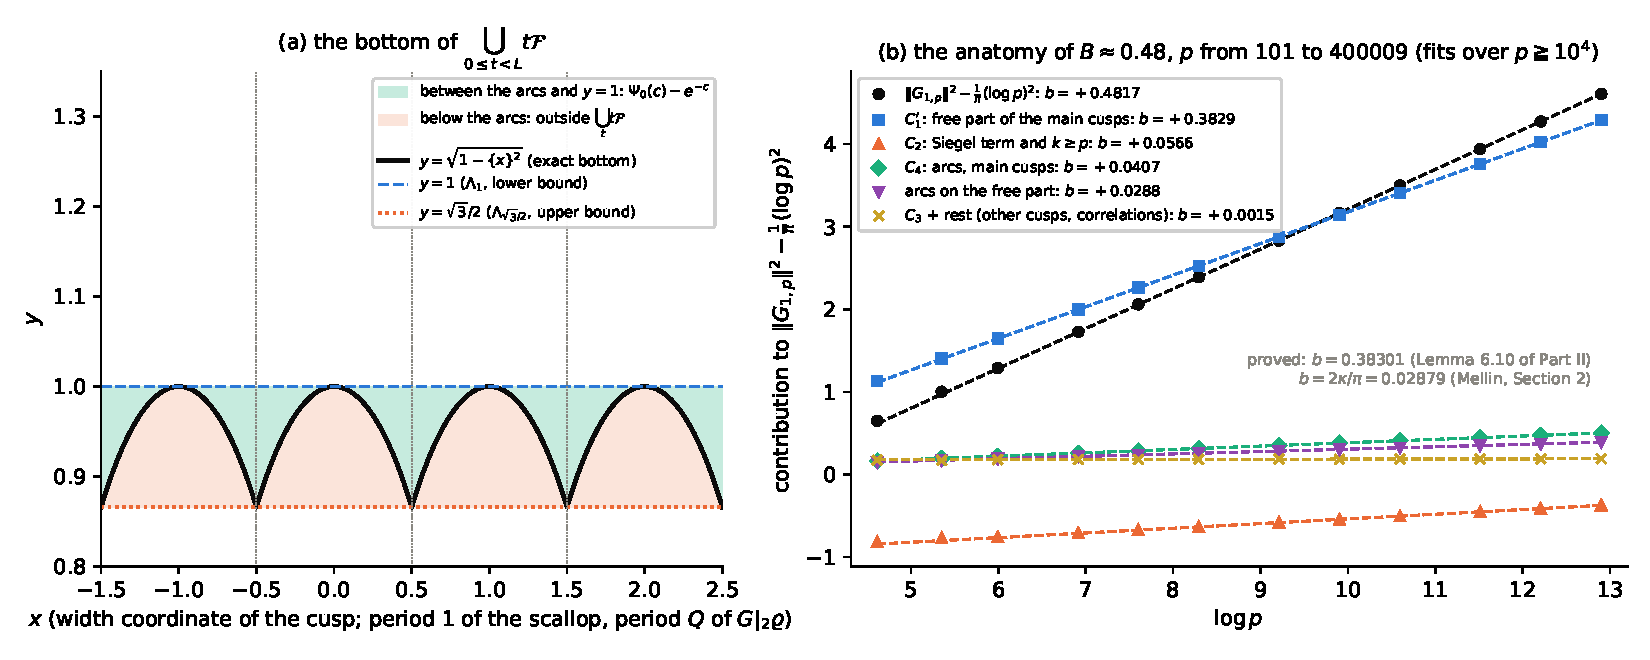
\includegraphics[width=\textwidth]{scalloped_anatomy.pdf}
\caption{(a) The lower boundary of $\bigcup_{0\le t<L}t\cF$ in the width coordinate of a cusp: the arcs $y=\sqrt{1-\{x\}^2}$, the line $y=1$ of the lower bound $\Lambda_1$ and the line $y=\sqrt3/2$ of the upper bound $\Lambda_{\sqrt3/2}$ of Part~II; the shaded region between the arcs and $y=1$ is what $\Psi_0(c)-e^{-c}$ integrates. (b) The parts of $\|G_{1,p}\|^2-\frac1\pi(\log p)^2$ against $\log p$ for the twelve primes of Table~\ref{tab:anatomy}, with their least-squares lines over $p\ge10^4$; the proved slopes of Theorem~\ref{thm:closedB} are listed. Script \texttt{plot\_scalloped\_anatomy.py}; floating point.}
\label{fig:anatomy}
\end{figure}

So $B\approx0.48$: $0.383$ and $0.029$ are proved by Mellin inversion, and the remaining $0.07$ is the Siegel and tail corrections at height $1$ ($0.057$) and through the arcs ($0.012$), plus the other cusps ($0.002$) and the correlations ($-0.0005$). These are not Mellin transforms of Dirichlet series, and the next subsection evaluates them by a different mechanism.

\subsection{The closed form of \texorpdfstring{$B$}{B}}\label{subsec:closedB}
For $k\ge p$ the coefficient is $a(k)=\sum_{\beta\ge0}r(\beta)r(k-p\beta)-M(k)$ with $r(0)=1$: the term $\beta=0$ is the free part $r(k)$, and $T'(k)=\sum_{\beta\ge1}r(\beta)r(k-p\beta)$ is the tail. In $|a(k)|^2$ the squares $r(k-p\beta)^2$, summed over $k$, produce a logarithm by $\sum_{a\le X}r(a)^2\sim4X\log X$; every other product is a shifted convolution of $r$, or involves the Siegel main term, and is bounded by the following elementary estimates.

\begin{lemma}\label{lem:elementary}
Uniformly for $X\ge1$ and integers $h\ge0$:
\begin{enumerate}[label=\textup{(\roman*)},leftmargin=2.2em]
\item for $h\ge1$, $\sum_{a\le X}r(a)r(a+h)\ll(X+h)\,\sigma_{-1}(h)+\sqrt{X+h}\,d(h)$;
\item $\sum_{a\le X}r(a)\sigma_{-1}(a+h)\ll X+h$ and $\sum_{a\le X}\sigma_{-1}(a)\sigma_{-1}(a+h)\ll X+h$;
\item $\sum_{a\le X}r(a)^2=4X\log X+O(X)$ and $\sum_{a\le X,\ a\equiv2\,(4)}r(a)^2=X\log X+O(X)$.
\end{enumerate}
\end{lemma}
\begin{proof}
(i) The sum counts $(x,y,z,w)\in\Z^4$ with $x^2+y^2\le X$ and $z^2+w^2-x^2-y^2=h$. The substitution $u_1=z-x$, $v_1=z+x$, $u_2=w-y$, $v_2=w+y$ is injective, gives $u_1v_1+u_2v_2=h$ and keeps $|u_i|,|v_i|\le U:=2\sqrt{X+h}$. If $u_1=0$, then $u_2v_2=h$ has at most $2d(h)$ solutions and $v_1$ at most $2U+1$ values; symmetrically for $u_2=0$; together $\ll Ud(h)$. If $u_1u_2\ne0$ and $g=(u_1,u_2)$, there is no solution unless $g\mid h$, and then $(v_1,v_2)$ runs over a coset of $\Z\,(u_2/g,-u_1/g)$, which has at most $1+2Ug/\max(|u_1|,|u_2|)$ points in the box. Summing over $(u_1,u_2)$, the $1$ gives $\ll U^2$, and with $u_i=gu_i'$, $(u_1',u_2')=1$, the second term gives $2U\sum_{g\mid h}\sum_{|u_i'|\le U/g}1/\max(|u_1'|,|u_2'|)\ll U\sum_{g\mid h}U/g=U^2\sigma_{-1}(h)$, as at most $8m$ pairs have $\max(|u_1'|,|u_2'|)=m$.

(ii) Write $\sigma_{-1}(a+h)=\sum_{e\mid a+h}1/e$ and split at $E=\log^2(2X+2h)$. The divisors $e>E$ contribute at most $E^{-1}\sum_{a\le X}r(a)d(a+h)\le E^{-1}\bigl(\sum_{a\le X}r(a)^2\bigr)^{1/2}\bigl(\sum_{n\le X+h}d(n)^2\bigr)^{1/2}\ll E^{-1}(X+h)\log^2(2X+2h)\ll X+h$. For $e\le E$, $\sum_{a\le X,\ e\mid a+h}r(a)$ counts the lattice points of the disc $x^2+y^2\le X$ in the $N_2(-h;e)$ residue classes modulo $e$ with $x^2+y^2\equiv-h$, so it is $N_2(-h;e)\bigl(\pi X/e^2+O(\sqrt X/e+1)\bigr)$ with $N_2(t;e)\le e\,d(e)^2$ (Part~II, proof of Lemma~6.4), and the sum over $e\le E$ is $\ll X\sum_ed(e)^2e^{-2}+\sqrt X\sum_{e\le E}d(e)^2e^{-1}+\sum_{e\le E}d(e)^2\ll X+h$. The second bound is the same argument with $r(a)$ replaced by $\sigma_{-1}(a)=\sum_{f\mid a}1/f$: for $e,f\le E$ the number of $a\le X$ with $f\mid a$, $e\mid a+h$ is at most $X(e,f)/(ef)+1$ and $\sum_{e,f}(e,f)(ef)^{-2}$ converges, while $e>E$ or $f>E$ contribute $\ll E^{-1}\sum_{a\le X}\bigl(d(a)\sigma_{-1}(a+h)+\sigma_{-1}(a)d(a+h)\bigr)\ll E^{-1}(X+h)\log^{2}(2X+2h)$ by Cauchy--Schwarz.

(iii) The first statement is Part~II, Lemma~6.3. For the second, $r(2m)=r(m)$ gives $\sum_{a\le X,\ a\ \mathrm{odd}}r(a)^2=R(X)-R(X/2)$ with $R(X)=\sum_{a\le X}r(a)^2$, and $a\equiv2\pmod4$ means $a=2m$ with $m$ odd, so the sum is $R(X/2)-R(X/4)=X\log X+O(X)$.
\end{proof}

\begin{theorem}[The closed form of $B$]\label{thm:closedB}
Let $E_1(x)=\int_x^\infty e^{-t}\,\dd t/t$, $s=\sqrt{1-x^2}$, $I_j(v_0;\lambda)=\int_{v_0}^\infty\Psi_j(\lambda v)\,\dd v/(\lambda v)$, and $r(0)=1$. Then
\[
\|G_{1,p}\|^2=\frac1\pi(\log p)^2+B\log p+O(1),\qquad B=b_1+b_2+b_3+b_4+b_5+b_6=0.48204\ldots,
\]
\begin{align*}
b_1&=\frac{c_1-2\log(4\pi^2)}{2\pi}=0.383005,\qquad b_2=\frac{2\kappa}\pi=0.028794,\\
b_3&=\frac1\pi\sum_{\beta\ge1}r(\beta)^2\bigl(E_1(\pi\beta)+E_1(4\pi\beta)\bigr)=0.056874,\\
b_4&=\frac1\pi\sum_{\beta\ge1}r(\beta)^2\int_{-1/2}^{1/2}\bigl(E_1(\pi\beta s)+E_1(4\pi\beta s)-E_1(\pi\beta)-E_1(4\pi\beta)\bigr)\dd x=0.011936,\\
b_5&=\frac1\pi\sum_{\beta\equiv2\,(4)}r(\beta)^2\int_{-1/2}^{1/2}E_1(\pi\beta s)\,\dd x=0.001893,\\
b_6&=\sum_{j\ge1}\Bigl[4\sum_{\beta\ge0}r(\beta)r(\beta+j)\,I_j(2\beta+j;2\pi)+2\sum_{\beta\ge0}r(\beta)r(\beta+4j)\,I_j(\beta+2j;\pi)\\
&\hskip4em+2\sum_{\beta\equiv2\,(4)}r(\beta)r(\beta+4j)\,I_j(\beta+2j;\pi)\Bigr]=-0.000460.
\end{align*}
Here $b_1$ is the free part of the two main cusps above height $1$ and $b_2$ the arcs on it (Section~\ref{sec:scallop}); $b_3$ and $b_4$ are the coefficients $k\ge p$ of the two main cusps above height $1$ and through the arcs; $b_5$ is the cusp of denominator $2$ (width $4p$) with its arcs; $b_6$ the correlation terms. The Siegel main term, all cross terms and the three narrow cusps contribute $O(1)$.
\end{theorem}
\begin{proof}
We go through the six classes of Proposition~\ref{prop:scallop}; $O(1)$ means bounded by a constant independent of $p$, and $M(k)\ll k\sigma_{-1}(k)/p$ uniformly in $k$ and $p$ by Part~II, Lemma~6.4 (the same for $M^{\mathrm{odd}}$).

\emph{The dominating estimate.} Every weight that occurs below has the form $F(t)=\phi(t/Y)/t$, up to a constant factor and a shift of $t$ by $jQ/2\ge0$, with $Y=Q/4\pi\asymp p$ and $\phi\in\{e^{-u},\ \Psi_0(u)-e^{-u},\ \Psi_j(u)\}$; all of these satisfy $|\phi(u)|,|\phi'(u)|\le2e^{-\sqrt3u/2}$ (for $\Psi_j$: $|\Psi_j'(u)|\le\int\sqrt{1-x^2}\,e^{-u\sqrt{1-x^2}}\dd x\le e^{-\sqrt3u/2}$, as $\sqrt{1-x^2}\ge\sqrt3/2$ on $[-\frac12,\frac12]$), so that $|F'(t)|\le2e^{-\sqrt3t/(2Y)}(1/(Yt)+1/t^2)$. Let $h\ge1$, let $c(a)$ be a sequence with $|c(0)|\ll d(h)$ and $\sum_{1\le a\le X}|c(a)|\ll(X+h)\sigma_{-1}(h)+\sqrt{X+h}\,d(h)$ for all $X\ge1$, and let $h'\ge\max(h,1)$. Then partial summation gives
\begin{multline}\label{eq:dominating}
\sum_{a\ge0}c(a)F(a+h')\ll\frac{d(h)}{h'}e^{-\sqrt3h'/(2Y)}+\int_{h'}^\infty\bigl(t\,\sigma_{-1}(h)+\sqrt t\,d(h)\bigr)e^{-\sqrt3t/(2Y)}\Bigl(\frac1{Yt}+\frac1{t^2}\Bigr)\dd t\\
\ll d(h)\Bigl(1+\frac Y{h'}\Bigr)e^{-\sqrt3h'/(2Y)}
\end{multline}
with an absolute implied constant: with $\lambda=\sqrt3/(2Y)$, $\int_{h'}^\infty e^{-\lambda t}(1/Y+1/t)\dd t=e^{-\lambda h'}/(\lambda Y)+E_1(\lambda h')\le e^{-\lambda h'}\bigl(2/\sqrt3+\log(1+1/(\lambda h'))\bigr)$ by $E_1(x)\le e^{-x}\log(1+1/x)$, $\int_{h'}^\infty e^{-\lambda t}(t^{-1/2}/Y+t^{-3/2})\dd t\le h'^{-1/2}e^{-\lambda h'}\bigl(1/(\lambda Y)+1/(\lambda h')\bigr)$, and $\sigma_{-1}(h)\le d(h)$. By Lemma~\ref{lem:elementary}(i) and (ii) the hypothesis holds for $c(a)=r(a)r(a+h)$ and for $c(a)=r(a)\sigma_{-1}(a+h)$. All $O(1)$ terms below are sums over $\beta,\beta'\ge1$ (and $j\ge1$) of bounds \eqref{eq:dominating} with $h'=p\max(\beta,\beta')$ and $Y\le p/\pi$, so that $Y/h'\le1/\pi$ and $h'/Y\ge\pi\max(\beta,\beta')$; and the resulting series converge uniformly in $p$, because $d(pn)\le2d(n)\le2n$ for a prime $p$ and $n\ge1$, together with $r(n)\le4d(n)\le4n$, gives
\[
\sum_{\beta\ne\beta'}r(\beta)r(\beta')\,d(p|\beta-\beta'|)\,e^{-\sqrt3\pi\max(\beta,\beta')/2}\le32\sum_{\beta,\beta'\ge1}\beta\beta'\max(\beta,\beta')\,e^{-\sqrt3\pi\max(\beta,\beta')/2}<\infty,
\]
and likewise on the diagonal $\beta=\beta'$ with $d(h)$ replaced by $1$. This is the uniformity in $p$; the same argument with $e^{-\sqrt3\pi\max(\beta,\beta')/2}$ replaced by $e^{-c\max(\beta,\beta')}$ for a fixed $c>0$ is what Section~\ref{subsec:oddasymp} uses.

\emph{Main cusps, height $1$.} At the width $Q\in\{p,4p\}$ the class is $\frac1{4\pi}\sum_k|a(k)|^2e^{-k/Y}/k$, $Y=Q/4\pi$, so $p\beta/Y=4\pi p\beta/Q\in\{4\pi\beta,\pi\beta\}\ge\pi\beta$. With $a=r+T'-M$, $|a|^2-r^2=2rT'+T'^2-2rM-2T'M+M^2$. By partial summation and Lemma~\ref{lem:elementary}(ii) with $h=0$, $\sum_kr(k)M(k)e^{-k/Y}/k\ll p^{-1}\sum_kr(k)\sigma_{-1}(k)e^{-k/Y}\ll Y/p\ll1$ and $\sum_kM(k)^2e^{-k/Y}/k\ll p^{-2}\sum_kk\sigma_{-1}(k)^2e^{-k/Y}\ll Y^2/p^2\ll1$. Next, $\sum_kr(k)T'(k)e^{-k/Y}/k=\sum_{\beta\ge1}r(\beta)\sum_{a\ge0}r(a)r(a+p\beta)F(a+p\beta)$ with $F(t)=e^{-t/Y}/t$, and \eqref{eq:dominating} with $h=h'=p\beta$ bounds the inner sum by $d(p\beta)e^{-\sqrt3\pi\beta/2}$, which sums to $O(1)$. Similarly $\sum_kT'(k)M(k)e^{-k/Y}/k\ll p^{-1}\sum_\beta r(\beta)\sum_ar(a)\sigma_{-1}(a+p\beta)e^{-(a+p\beta)/Y}\ll p^{-1}\sum_\beta r(\beta)(Y+p\beta)e^{-\pi\beta}\ll1$ by (ii) and partial summation. In $T'(k)^2=\sum_{\beta,\beta'\ge1}r(\beta)r(\beta')r(k-p\beta)r(k-p\beta')$ the terms $\beta<\beta'$ are, with $k=a+p\beta'$, the sums $\sum_{a\ge0}r(a)r(a+p(\beta'-\beta))F(a+p\beta')$, and \eqref{eq:dominating} with $h=p(\beta'-\beta)$, $h'=p\beta'$ bounds them by $d(p(\beta'-\beta))e^{-\sqrt3\pi\beta'/2}$: again $O(1)$ in total. The diagonal $\beta=\beta'$ is
\[
D_Q=\sum_{\beta\ge1}r(\beta)^2\sum_{a\ge0}r(a)^2\,\frac{e^{-(a+p\beta)/Y}}{a+p\beta},
\]
and by (iii) and partial summation, $\sum_{a\ge1}r(a)^2F(a+h)=\int_1^\infty(4X\log X+O(X))(-F'(X+h))\,\dd X$ for $F(t)=e^{-t/Y}/t$, where $-F'(t)=e^{-t/Y}(1/(Yt)+1/t^2)>0$; the $O(X)$ part is $\ll e^{-h/Y}+E_1(h/Y)\ll e^{-h/2Y}$, and the main part is, after an integration by parts and $X=Yu$,
\[
4\int_1^\infty(\log X+1)\frac{e^{-(X+h)/Y}}{X+h}\,\dd X=4\log Y\,E_1(h/Y)+O(e^{-h/2Y}).
\]
With $h=p\beta$, $\log Y=\log p+O(1)$ and $h/Y\ge\pi\beta$, this gives $D_Q=4\log p\sum_\beta r(\beta)^2E_1(4\pi p\beta/Q)+O(1)$, and $\frac1{4\pi}(D_p+D_{4p})=b_3\log p+O(1)$.

\emph{Main cusps, arcs.} The terms $j=0$ with $\Psi_0(c)-e^{-c}$ in place of $e^{-c}$ are treated identically: the weight is $F(t)=(\Psi_0(t/Y)-e^{-t/Y})/t$, to which \eqref{eq:dominating} applies as it stands, and in the diagonal $\int_0^\infty\Psi_0(u+v_0)\,\dd u/(u+v_0)=\int_{-1/2}^{1/2}E_1(sv_0)\,\dd x$ by Fubini, since $\int_0^\infty e^{-s(u+v_0)}\dd u/(u+v_0)=E_1(sv_0)$. Subtracting $E_1(v_0)$ gives $b_4$.

\emph{Main cusps, correlations.} For $j\ge1$ the term is $\frac2Q\sum_ka(k)a(k+jQ)\Psi_j(c)/c$ with $c=2\pi(2k+jQ)/Q=(k+jQ/2)/Y$, i.e.\ the weight $\frac1{2\pi}F(k+jQ/2)$ with $F(t)=\Psi_j(t/Y)/t$. Expanding both factors, every product containing $M$ or two different arguments of $r$ is bounded by \eqref{eq:dominating} (the shift $jQ/2$ only increases $h'$, and $jQ/(2Y)=2\pi j$), giving $O(e^{-\sqrt3\pi j})$ with geometric decay in $\beta,\beta'$. The squares $r(k-p\beta)^2$ occur exactly when $\beta'-\beta=jQ/p$: $\beta'=\beta+j$ for $Q=p$ and $\beta'=\beta+4j$ for $Q=4p$, now with $\beta\ge0$, the term $\beta=0$ being the free part $r(k)$ paired with the term $\beta'=jQ/p$ of the tail. With $k=a+p\beta$, $a=pu$, partial summation with (iii) gives $\sum_ar(a)^2\Psi_j(c)/c=4p\log p\int_0^\infty\Psi_j(c(u))\,\dd u/c(u)+O(p)$, where $c(u)=2\pi(2u+2\beta+j)$ for $Q=p$ and $c(u)=\pi(u+\beta+2j)$ for $Q=4p$; the integrals are $\frac12I_j(2\beta+j;2\pi)$ and $I_j(\beta+2j;\pi)$, and with the factors $2/Q$ the two widths give $4\log p\sum_\beta r(\beta)r(\beta+j)I_j(2\beta+j;2\pi)$ and $2\log p\sum_\beta r(\beta)r(\beta+4j)I_j(\beta+2j;\pi)$: the first two sums of $b_6$.

\emph{The cusp of denominator $2$.} Its width is $4p$, $w_d=p$ and $b=\frac1p(T^{\mathrm{odd}}-M^{\mathrm{odd}})$ (Part~II, Lemma~6.12), where $T^{\mathrm{odd}}(k)=\sum_{\beta\ge1}r^{\mathrm{o}}(\beta)r^{\mathrm{o}}(k-p\beta)$ with $r^{\mathrm{o}}(a)=r(a)$ for $a\equiv2\pmod4$ and $0$ otherwise (odd $x,y$ force $x^2+y^2\equiv2\pmod8$, and conversely). The class is $\frac1\pi\sum_k(T^{\mathrm{odd}}-M^{\mathrm{odd}})^2(k)e^{-\pi k/p}/k$ (height $1$) and the same with $\Psi_0-e^{-c}$; there is no free part, the $M^{\mathrm{odd}}$ terms and the off-diagonal terms are $O(1)$ as above, and the diagonal gives, by the second part of (iii) (coefficient $1$ in place of $4$) and $Y=p/\pi$, $\frac1\pi\log p\sum_{\beta\equiv2(4)}r(\beta)^2\int E_1(\pi\beta s)\dd x+O(1)=b_5\log p+O(1)$, height $1$ and arcs together. Its correlations are the third sum of $b_6$, by the computation for $Q=4p$.

\emph{The narrow cusps.} At the widths $4$ and $1$ the weights are $e^{-\pi k}$ and $e^{-4\pi k}$; the coefficients are $a(k)=r(k)-M(k)$ for $k<p$ with $M(k)\ll k\sigma_{-1}(k)/p$, so these classes are $\frac1{4\pi}\sum_kr(k)^2e^{-4\pi k/Q}/k+O(1/p)$, and the cusp of denominator $2p$ has $T^{\mathrm{odd}}(1,p;k)=0$ for $k<2(p+1)$ (Part~II, Lemma~6.12), hence is $O(1/p)$ as well; the same holds for their arc and correlation terms.

Adding $b_1$ (Lemma~6.3 of Part~II, as in Section~\ref{subsec:anatomy}) and $b_2$ (Proposition~\ref{prop:mellin}) gives the theorem. The script \texttt{closed\_form\_B.py} evaluates $b_1,\dots,b_6$ ($E_1$ from \texttt{scipy}, the $x$- and $v$-integrals by quadrature, $\beta\le40$, $j\le8$) and compares them with the local slopes of the exact anatomy over $p=2\cdot10^5$, $4\cdot10^5$: $0.05687/0.05676$ ($C_2$), $0.00133/0.00134$ (cusp of denominator $2$ at height $1$), $0.04073/0.04073$ (arcs, main cusps), $0.00057/0.00058$ (arcs, other cusps), $-0.00046/-0.00046$ (correlations) and $0.48204/0.48188$ for the total; and the part of $C_2$ that remains after the diagonal is removed is $-1.1691\pm0.0001$ at height $1$ and $-0.05762$ through the arcs for all $10^4\le p\le4\cdot10^5$.
\end{proof}

\begin{remark}
(a) The Siegel main term does not enter $B$: the sums $\sum r(k)\beta(k)$ and $\sum\beta(k)^2$ grow linearly, without a logarithm, which is Lemma~\ref{lem:elementary}(ii) and sharpens Part~II, Lemma~6.4, by the factor $\log 2Y$ there. The whole of $B-b_1-b_2=0.0702$ comes from the squares $r(k-p\beta)^2$, $\beta\ge1$, i.e.\ from the representations $k=\alpha+p\beta$ of the coefficients $k\ge p$, through the exponential integral $E_1(4\pi p\beta/Q)$ of the position $p\beta/Y$ of the shifted copy of $\sum r(a)^2$ in the weight $e^{-k/Y}$; the terms $\beta=1,2$ carry all but $10^{-6}$ of it. (b) The same mechanism applies to the odd Heegner discriminants of Section~\ref{sec:heegner}, where $\sum_{a\le X}r_D(a)^2=\frac{24}{D+1}X\log X+O(X)$: at the two wide cusps (widths $Dp$ and $p$, so $4\pi p\beta/Q\in\{4\pi\beta/D,4\pi\beta\}$) the tail adds $\frac{6}{\pi(D+1)}\sum_{\beta\ge1}r_D(\beta)^2\bigl(E_1(4\pi\beta/D)+E_1(4\pi\beta)\bigr)\log p$, which for $D=4$ is $b_3$. Section~\ref{subsec:oddasymp} carries this out: Lemma~\ref{lem:elementaryD} is the analogue of Lemma~\ref{lem:elementary} for the form $N_D$, and Theorem~\ref{thm:closedBD} the closed form of $B_D$.
\end{remark}

\section{The theta series of the odd Heegner discriminants}\label{sec:heegner}

\subsection{Setting}
Let $D$ be one of the seven odd Heegner discriminants (the nine imaginary quadratic fields of class number one have $D\in\{3,4,7,8,11,19,43,67,163\}$, Heegner--Stark \cite{Stark}), $K=\Q(\sqrt{-D})$, $\chi=\chi_{-D}$ the Kronecker symbol, $w_D$ the number of units ($w_3=6$, $w_D=2$ otherwise), $N_D(x,y)=x^2+xy+\frac{D+1}4y^2$ (Gram determinant $D$), $r_D(n)=\#\{N_D=n\}=w_D\sum_{d\mid n}\chi(d)$ for $n\ge1$ (class number one), and $\theta_D(z)=\sum_{n\ge0}r_D(n)e(nz)\in M_1(\Gamma_0(D),\chi)$. The Eisenstein series $E(z,s)=\sum_{\Gamma_\infty\backslash\Gamma_0(D)}\chi(d_\gamma)j(\gamma,z)^{-1}\operatorname{Im}(\gamma z)^s$ has at $s=0$ the expansion $1+\frac2{L(0,\chi)}\sum\sigma_\chi(n)e(nz)$ with $L(0,\chi)=2h/w_D=2/w_D$ (Hecke; see \cite[Chapter~4]{DS} for the weight-one Eisenstein series), so $E(z,0)=\theta_D$ without any dimension argument. For a prime $p\ne D$, $\Theta_{1,p}=\theta_D(z)\theta_D(pz)=E+G\in M_2(\Gamma_0(Dp))$, $T(k)=\sum_{\alpha+p\beta=k}r_D(\alpha)r_D(\beta)$, $a_G(k)=T(k)-M(k)$. The level $Dp$ is square-free: $\Gamma_0(Dp)$ has the four cusps $W_Q\infty$, $Q\in\{1,D,p,Dp\}$, of widths $Dp,p,D,1$, and no cusp of denominator $2\delta$. We write $|_k$ for the weight-$k$ slash operator normalised by $(\det\gamma)^{k/2}$, so that scalars act trivially and $f(mz)=m^{-k/2}(f|_kB_m)(z)$, $B_m=\left(\begin{smallmatrix}m&0\\0&1\end{smallmatrix}\right)$.

\subsection{The Siegel main term}
\begin{theorem}\label{thm:siegel}
$M(k)=\dfrac{4\pi^2k}{Dp}\prod_\ell\beta_\ell(k)$, where $\beta_\ell(k)=(1-\ell^{-2})\sigma_{-1}(\ell^{v_\ell(k)})$ for every prime $\ell\nmid Dp$, including $\ell=2$, and, with $v=v_\ell(k)$,
\[
\beta_p(k)=(1+\chi(p))-\chi(p)\Bigl(1+\frac1p\Bigr)p^{-v},\qquad \beta_D(k)=(1+\e)-\e\Bigl(1+\frac1D\Bigr)D^{-v},
\]
where $\e=\bigl(\frac{-p}D\bigr)=-\chi_{-D}(p)$. Explicitly, with $v=v_\ell(k)$:
\begin{center}\footnotesize
\begin{tabular}{l|ccc}
\toprule
 & $\ell\nmid Dp$ & $\ell=p$ (sign $\chi(p)$) & $\ell=D$ (sign $\e=-\chi(p)$)\\
\midrule
$v=0$ & $1-\ell^{-2}$ & $1-\chi(p)/p$ & $1-\e/D$\\
$v\ge1$, sign $+1$ & $(1-\ell^{-2})\sigma_{-1}(\ell^v)$ & $2-(1+1/p)p^{-v}$ & $2-(1+1/D)D^{-v}$\\
$v\ge1$, sign $-1$ & $(1-\ell^{-2})\sigma_{-1}(\ell^v)$ & $(1+1/p)p^{-v}$ & $(1+1/D)D^{-v}$\\
\bottomrule
\end{tabular}
\end{center}
The rows $v\ge1$ follow from the recursions $\beta_p(k)=(1+\chi(p))(1-1/p)+\beta_p(k/p)/p$ and $\beta_D(k)=(1+\e)(1-1/D)+\beta_D(k/D)/D$ of the proof, iterated $v$ times from the row $v=0$. In particular $\beta_\ell(k)\le4\sigma_{-1}(\ell^{v})$ at every prime, so $M(k)\ll k\sigma_{-1}(k)/(Dp)$ uniformly in $k$, $p$ and $D$.
\end{theorem}
\begin{proof}
The quaternary form $Q=N_D(x,y)+pN_D(z,w)$ has Gram determinant $D^2p^2$, and Siegel's theorem \cite{Siegel} (see \cite[Chapter~6]{Kitaoka} for the local densities) gives $r(\gen Q,k)=4\pi^2k\prod_\ell\beta_\ell(k)/\sqrt{D^2p^2}$ with $\beta_\ell(k)=\lim_a\ell^{-3a}\#\{x\bmod\ell^a:\ Q(x)\equiv k\}$; the genus theta series is the Eisenstein part of $\Theta_{1,p}$. For $\ell\nmid Dp$ the form is unimodular over $\Z_\ell$ with square discriminant, which gives the standard density; this includes $\ell=2$ because $N_D$ is even unimodular over $\Z_2$, $pN_D\cong N_D$ there ($p$ a unit; the Arf invariant is insensitive to unit scaling), and $N_D\oplus N_D$ has Arf invariant $0$, i.e.\ is the sum of two hyperbolic planes, whatever the class of $N_D$ modulo $2$.

At $\ell=p$: the solutions with $(x,y)\not\equiv(0,0)\pmod p$ are non-singular in $(x,y)$, so each solution modulo $p$ lifts to $p^{a-1}$ solutions modulo $p^a$; modulo $p$ the equation $N_D(x,y)\equiv t$ has $p-\chi(p)$ solutions for $p\nmid t$ and $1+(p-1)(1+\chi(p))$ for $p\mid t$. With $(z,w)$ free this gives $\beta_p(k)=1-\chi(p)/p$ for $p\nmid k$ and the contribution $(1+\chi(p))(1-1/p)$ for $p\mid k$. The solutions with $x\equiv y\equiv0\pmod p$, $x=px'$, $y=py'$, satisfy $pN_D(x',y')+N_D(z,w)\equiv k/p\pmod{p^{a-1}}$, the same form with the blocks interchanged; counting $(x',y')$ modulo $p^{a-1}$ and the $p^2$ lifts of $(z,w)$ gives $\beta_p(k/p)/p$. Hence $\beta_p(k)=(1+\chi(p))(1-1/p)+\beta_p(k/p)/p$ for $p\mid k$, which iterates to the closed form.

At $\ell=D$: since $2$ is invertible, $N_D(x,y)=(x+y/2)^2+\frac D4y^2\cong u^2+Dv^2$ over $\Z_D$, so $Q\cong u^2+ps^2+D(v^2+pt^2)$. The solutions with $(u,s)\not\equiv0\pmod D$ are non-singular in $(u,s)$; modulo $D$ the binary form $u^2+ps^2$, of discriminant $-4p$, represents $t\not\equiv0$ exactly $D-\e$ times and $t\equiv0$ exactly $1+(D-1)(1+\e)$ times, $\e=(-p/D)$. The solutions with $u\equiv s\equiv0$ reduce to $D(u'^2+ps'^2)+(v^2+pt^2)\equiv k/D\pmod{D^{a-1}}$, the same form, with the factor $D^2/D^3=1/D$. Hence $\beta_D(k)=1-\e/D$ for $D\nmid k$ and $\beta_D(k)=(1+\e)(1-1/D)+\beta_D(k/D)/D$ for $D\mid k$. Finally $(-p/D)=(-1/D)(p/D)=-(p/D)=-(-D/p)=-\chi_{-D}(p)$ by quadratic reciprocity, $D\equiv3\pmod4$.
\end{proof}

\subsection{Atkin--Lehner signs and the spectral support}\label{subsec:support}
\begin{theorem}\label{thm:AL}
$\Theta_{1,p}|_2W_p=\chi(p)\Theta_{1,p}$, $\Theta_{1,p}|_2W_D=-\chi(p)\Theta_{1,p}$ and $\Theta_{1,p}|_2W_{Dp}=-\Theta_{1,p}$, for any choice of the Atkin--Lehner matrices \cite{AL} of level $Dp$.
\end{theorem}
\begin{proof}
Write $W_p=\left(\begin{smallmatrix}pa&b\\Dpc&pd\end{smallmatrix}\right)$, $pad-Dbc=1$. Then $W_p=\gamma B_p$ with $\gamma=\left(\begin{smallmatrix}a&b\\Dc&pd\end{smallmatrix}\right)\in\Gamma_0(D)$, so $\theta_D|_1W_p=\chi(pd)p^{1/2}\theta_D(pz)$; and $B_pW_p=p\left(\begin{smallmatrix}pa&b\\Dc&d\end{smallmatrix}\right)$ with the second factor in $\Gamma_0(D)$, so $\theta_D(p\,\cdot)|_1W_p=p^{-1/2}\chi(d)\theta_D$. The product is $\chi(p)\Theta_{1,p}$.

For $W_D$: the dual of the lattice $(\mathcal O_K,N_D)$ is $\mathcal O_K/\sqrt{-D}$, so Poisson summation gives $\theta_D(-1/z)=D^{-1/2}(-iz)\theta_D(z/D)$ and $\theta_D(-1/(Dz))=-i\sqrt Dz\,\theta_D(z)$, i.e.\ $\theta_D|_1W_0=-i\theta_D$ for $W_0=\left(\begin{smallmatrix}0&-1\\D&0\end{smallmatrix}\right)$. Every matrix $W=\left(\begin{smallmatrix}Da'&b'\\Dc'&Dd'\end{smallmatrix}\right)$ of determinant $D$ is $W_0\gamma'$ with $\gamma'=\left(\begin{smallmatrix}c'&d'\\-Da'&-b'\end{smallmatrix}\right)\in\Gamma_0(D)$, whence $\theta_D|_1W=-i\chi(-b')\theta_D$. Now $W_D=\left(\begin{smallmatrix}Da&b\\Dpc&Dd\end{smallmatrix}\right)$, $Dad-pbc=1$, is such a matrix with $b'=b$, and $B_pW_D=\left(\begin{smallmatrix}Da&pb\\Dc&Dd\end{smallmatrix}\right)B_p$ exhibits $\theta_D(p\,\cdot)|_1W_D=p^{-1/2}(\theta_D|_1W')|_1B_p$ with $W'$ such a matrix with $b'=pb$. Therefore $\Theta_{1,p}|_2W_D=(-i)^2\chi(-b)\chi(-pb)\Theta_{1,p}=-\chi(p)\Theta_{1,p}$, using $(b,D)=1$; and $W_{Dp}\equiv W_DW_p$ modulo $\Gamma_0(Dp)$ gives $-1$.
\end{proof}

\begin{theorem}[Spectral support]\label{thm:support}
Let $\varphi$ be a newform of weight $2$ and level $Dp$. If $\langle\Theta_{1,p},\varphi\rangle\ne0$ then $\eta_p(\varphi)=\chi(p)$, $\eta_D(\varphi)=-\chi(p)$, i.e.\ $a_\varphi(D)=\chi_{-D}(p)$, $a_\varphi(p)=-\chi_{-D}(p)$, and the root number of $\varphi$ is $+1$. For a newform $f$ of level $p$ and $d\mid D$, $\langle\Theta_{1,p},f(d\,\cdot)\rangle\ne0$ requires $\eta_p(f)=\chi(p)$, i.e.\ $a_f(p)=-\chi_{-D}(p)$. For a newform $f$ of level $D$ and $d\mid p$, $\langle\Theta_{1,p},f(d\,\cdot)\rangle=C_D(1+\chi(p))L(1,f)L(1,f\otimes\chi)/d$ vanishes when $\chi_{-D}(p)=-1$.
\end{theorem}
\begin{proof}
$\langle\Theta,\varphi\rangle=\langle\Theta|W,\varphi|W\rangle$ for $W=W_p,W_D$ and Theorem~\ref{thm:AL} give $\chi(p)\eta_p(\varphi)=1$ and $-\chi(p)\eta_D(\varphi)=1$; $a_\varphi(\ell)=-\eta_\ell(\varphi)$ for $\ell\,\|\,Dp$, and the root number is $-\eta_D\eta_p$. For $f$ of level $p$, Part~II, Lemma~6.8 (with $Q=p$) gives $f(d\,\cdot)|_2W_p=\eta_p(f)f(d\,\cdot)$, and the same argument applies; $W_D$ exchanges $f(z)$ and $f(Dz)$ up to a factor and gives no further condition. For $f$ of level $D$ the formula is the oldform computation in the proof of Part~II, Theorem~6.7(ii), with $D$ in the role of $4$ and $p$ in the role of $n$: the brackets there give $\sum_{Q_2\mid d}\chi(Q_2)\prod_{\ell\mid p/d}(1+\chi(\ell))=1+\chi(p)$ in both cases $d=1,p$.
\end{proof}

Theorem~\ref{thm:support} gives necessary conditions. What is proved about the actual support, and what is only observed, is the following.

\begin{proposition}\label{prop:whatproved}
Let $\mathcal S(D,p)$ be the set of newforms $\varphi$ of weight $2$ and level $Dp$ with $\eta_p(\varphi)=\chi(p)$ and $\eta_D(\varphi)=-\chi(p)$.
\begin{enumerate}[label=\textup{(\roman*)},leftmargin=2.2em]
\item The newform part of $G^{(D)}_{1,p}$ lies in the span of $\mathcal S(D,p)$ (Theorem~\ref{thm:support}), and for $\varphi\in\mathcal S(D,p)$ one has $\langle\Theta_{1,p},\varphi\rangle\ne0$ if and only if $L(1,\varphi)L(1,\varphi\otimes\chi_{-D})\ne0$ (Theorem~\ref{thm:RS} below). Both central values have root number $+1$ in this situation, and their non-vanishing is not addressed here.
\item In contrast with $D=4$, where every newform of level $4n$ has $\eta_4=-1$ (Part~II, Proposition~6.17), so that the newform support is empty whenever $\chi_{-4}(n)=-1$, neither sign of $W_D$ is excluded at the square-free level $Dp$: the local component at $D$ is the Steinberg representation or its unramified quadratic twist, and both occur. $\mathcal S(D,p)$ has dimension $\frac14(\dim S^{\mathrm{new}}+\chi(p)\tr W_p-\chi(p)\tr W_D-\tr W_{Dp})$, the traces taken on $S_2^{\mathrm{new}}(\Gamma_0(Dp))$; these traces are sums of class numbers of size $O_\e((Dp)^{1/2+\e})$ by the trace formulae for the Atkin--Lehner involutions (Yamauchi \cite{Yamauchi} for the Fricke involution; Martin \cite{Martin} for the eigenspaces with prescribed signs at square-free level), so $\#\mathcal S(D,p)$ is asymptotically a quarter of the new subspace, half of the forms with root number $+1$. Nothing in this paper depends on this count.
\item \emph{Observed} (Section~\ref{sec:num}): for $D\le43$ and the primes tested, every newform component of $G^{(D)}_{1,p}$ found by the Hecke decomposition lies in $\mathcal S(D,p)$ ($91$ components). The converse, whether every $\varphi\in\mathcal S(D,p)$ occurs, i.e.\ whether $L(1,\varphi)L(1,\varphi\otimes\chi_{-D})\ne0$ for all of them, has not been tested: the decomposition of $G$ finds only the forms that do occur.
\end{enumerate}
\end{proposition}

The oldforms from level $D$ exist for $D\in\{11,19,43,67,163\}$ (genus $1,1,3,5,13$) and not for $D=3,7$; at the level $22$ ($\chi_{-11}(2)=-1$) the cuspidal part vanishes identically, $\theta_{11}(z)\theta_{11}(2z)=E$, while at the level $55$ ($\chi_{-11}(5)=+1$) the component of $f_{11}$ is $f_{11}(z)+5f_{11}(5z)$ up to a scalar and carries $25\%$ of the norm.

\subsection{The Rankin--Selberg formula}
\begin{theorem}\label{thm:RS}
For a newform $\varphi$ of weight $2$ and level $Dp$,
\[
\langle\Theta_{1,p},\varphi\rangle=C_D\,\chi(p)\,\eta_p(\varphi)\,L(1,\varphi)\,L(1,\varphi\otimes\chi_{-D}),\qquad C_D=\frac{w_D}{4\pi L(1,\chi_{-D})}=\frac{w_D^2\sqrt D}{8\pi^2};
\]
$C_3=\frac{9\sqrt3}{2\pi^2}=0.7897$, $C_D=\frac{\sqrt D}{2\pi^2}$ for $D\ge7$, against $C_4=\frac4{\pi^2}$ and $C_8=\frac{\sqrt2}{\pi^2}$.
\end{theorem}
\begin{proof}
The proof of Part~II, Theorem~6.7(i) carries over: $\theta_D=E(z,0)$; the cusps of $\Gamma_0(Dp)$ over $\infty$ of $\Gamma_0(D)$ are $W_Q\infty$, $Q\mid p$; unfolding gives $I(s)=\sum_{Q\mid p}\chi(Q)\Gamma(s+1)(4\pi)^{-s-1}\sum_{j}r_D(j)c_Q((p/Q)j)((p/Q)j)^{-s-1}$, with $\chi(a)\chi(d)=\chi(Q)$ from $Qad\equiv1\pmod D$ and $c_Q(k)=\eta_Q(\varphi)a_\varphi(k)$; the Dirichlet series $\sum_jr_D(j)a_\varphi(j)j^{-w}=w_D\sum_j\sigma_\chi(j)a_\varphi(j)j^{-w}$ is $w_DL(w,\varphi)L(w,\varphi\otimes\chi)/(L(2w-1,\chi)\prod_{\ell\mid p}(1-\chi(\ell)\ell^{1-2w}))$. Here $L(w,\varphi)=\sum_na_\varphi(n)n^{-w}$ with $a_\varphi(1)=1$, so that the central point is $w=1$, $L(w,\varphi\otimes\chi)=\sum_n\chi(n)a_\varphi(n)n^{-w}$, and the Euler factors are, with $x=\ell^{-w}$: for $\ell\nmid Dp$ the Rankin--Selberg factor $\sum_j\sigma_\chi(\ell^j)a_\varphi(\ell^j)x^j=(1-\chi(\ell)\ell x^2)L_\ell(w,\varphi)L_\ell(w,\varphi\otimes\chi)$ (Part~II, Theorem~6.7, with $\alpha\beta=\ell$); for $\ell=p$, where $a_\varphi(p^j)=a_\varphi(p)^j$, the factor $\sum_j\sigma_\chi(p^j)a_\varphi(p)^jx^j=(1-a_\varphi(p)x)^{-1}(1-\chi(p)a_\varphi(p)x)^{-1}=L_pL_p$ without the numerator, which is why the factor $\ell=p$ of $1/L(2w-1,\chi)$ is divided out; and for $\ell=D$, where $\chi(D)=0$, $\sigma_\chi(D^j)=1$ and $a_\varphi(D^j)=a_\varphi(D)^j$, the factor $\sum_ja_\varphi(D)^jx^j=(1-a_\varphi(D)x)^{-1}=L_D(w,\varphi)L_D(w,\varphi\otimes\chi)$, the twisted factor at $D$ being $1$. At $s=0$ the constant is $w_D/(4\pi L(1,\chi))$, and $\sum_{Q\mid p}\chi(Q)\eta_Q(\varphi)a_\varphi(p/Q)/(p/Q)=\chi(p)\eta_p(\varphi)(1-\chi(p)/p)$ cancels the local factor. The class number formula $L(1,\chi_{-D})=2\pi h/(w_D\sqrt D)$ with $h=1$ gives the second expression.
\end{proof}

\subsection{The norm}
\begin{theorem}\label{thm:norm}
Let $D_D(s)=\sum_kr_D(k)^2k^{-s}$. Then $D_D(s)=w_D^2\,\zeta(s)^2L(s,\chi)^2/\bigl((1+D^{-s})\zeta(2s)\bigr)$ and
\begin{gather*}
S_D(Y):=\sum_{k\ge1}\frac{r_D(k)^2}k e^{-k/Y}=\frac{12}{D+1}(\log Y)^2+c_1^{(D)}\log Y+c_2^{(D)}+O(Y^{-1/2}),\\
c_1^{(D)}=\frac{24}{D+1}\Bigl(\gamma+2\frac{L'}L(1,\chi)-2\frac{\zeta'}\zeta(2)+\frac{\log D}{D+1}\Bigr),\\
\frac{L'}L(1,\chi_{-D})=\gamma+\log2+\log\pi-\frac{w_D}2\sum_{a=1}^{D-1}\chi(a)\log\Gamma\Bigl(\frac aD\Bigr).
\end{gather*}
Consequently the regions above height $1$ at the two wide cusps give
\begin{gather*}
\|G^{(D)}_{1,p}\|^2\ \ge\ \frac1{4\pi}\Bigl(S_D\Bigl(\frac{Dp}{4\pi}\Bigr)+S_D\Bigl(\frac p{4\pi}\Bigr)\Bigr)+O(1)=\frac6{\pi(D+1)}(\log p)^2+b_D\log p+O(1),\\
b_D=\frac{6}{\pi(D+1)}\log\frac D{16\pi^2}+\frac{c_1^{(D)}}{2\pi},
\end{gather*}
with $b_3=0.713$, $b_7=0.207$, $b_{11}=0.133$, $b_{19}=0.121$, $b_{43}=0.143$, $b_{67}=0.150$, $b_{163}=0.142$.
\end{theorem}
\begin{proof}
$r_D/w_D=\sigma_\chi$ is multiplicative with $\sigma_\chi(\ell^j)=j+1$, $\frac12(1+(-1)^j)$, $1$ for $\chi(\ell)=1,-1,0$, so the Euler factor of $\sum\sigma_\chi(k)^2k^{-s}$ at $\ell\ne D$ is that of $\zeta^2L^2/\zeta(2s)$, and at $\ell=D$ it is $(1-x)^{-1}$ against $(1+x)/(1-x)$, whence the factor $(1+D^{-s})^{-1}$. At $s=1$: $w_D^2L(1,\chi)^2\cdot\frac D{D+1}\cdot\frac6{\pi^2}=\frac{24}{D+1}$ by the class number formula. Mellin inversion, $S_D(Y)=\frac1{2\pi i}\int_{(2)}\Gamma(s)D_D(1+s)Y^s\,\dd s$, with the contour moved to $\operatorname{Re}s=-\frac12$ across the double pole at $s=0$ ($L(1+s,\chi)^2$ is entire, $1/\zeta(2+2s)$ is holomorphic and of polynomial growth for $\operatorname{Re}s\ge-\frac12$, and $\Gamma(s)$ decays exponentially), gives $S_D(Y)$ with the residue $\frac{12}{D+1}(\log Y)^2+c_1^{(D)}\log Y+c_2^{(D)}$, exactly as in Part~II, Lemma~6.3, where $c_1^{(D)}=\frac{24}{D+1}(\gamma+a_1)$ with $a_1$ the coefficient of $s$ in $D_D(1+s)\cdot\frac{D+1}{24}s^2=1+a_1s+\dots$, i.e.\ $a_1=2\gamma+2\frac{L'}L(1,\chi)-2\frac{\zeta'}\zeta(2)+\frac{\log D}{D+1}$. The value of $\frac{L'}L(1,\chi)$ follows from the functional equation $\Lambda(s)=(D/\pi)^{s/2}\Gamma(\frac{s+1}2)L(s,\chi)=\Lambda(1-s)$ and $L(s,\chi)=D^{-s}\sum_a\chi(a)\zeta(s,a/D)$ with $\zeta'(0,a)=\log\Gamma(a)-\frac12\log2\pi$: $\frac{L'}L(1)=-\log\frac D\pi-\frac12\psi(\frac12)-\frac12\psi(1)-\frac{L'}L(0)$ and $\frac{L'}L(0)=-\log D+\frac{w_D}2\sum_a\chi(a)\log\Gamma(a/D)$, since $L(0,\chi)=2/w_D$. The lower bound for the norm is Part~II, Lemma~6.2 at the cusps $W_1\infty$ and $W_D\infty$ (widths $Dp$ and $p$), which carry $\pm G_{1,p}$ by Theorem~\ref{thm:AL}: the regions $y\ge1$ there contribute $\frac1{4\pi}\sum_k|a(k)|^2k^{-1}e^{-4\pi k/Q}$, $Q\in\{Dp,p\}$, and the difference between $|a(k)|^2$ and $r_D(k)^2$ (the Siegel main term and the coefficients $k\ge p$) contributes $O(1)$ plus the non-negative tail term $b_3^{(D)}\log p$ by Lemma~\ref{lem:elementaryD} and the proof of Theorem~\ref{thm:closedBD} below.
\end{proof}

\subsection{The asymptotic formula for the odd discriminants}\label{subsec:oddasymp}
The level $Dp$ is square-free, so Proposition~\ref{prop:scallop} has four classes, all Atkin--Lehner, of widths $Q\in\{Dp,p,D,1\}$, each with $w_d=Q$ and $b=\pm a_G/Q$ (Theorem~\ref{thm:AL} and the computation of Part~II, Lemma~6.2, whose pair count $\varphi(L)Q$ holds for every square-free $L$): the class of width $Q$ is $\frac1Q\sum_{k,j}a(k)a(k+jQ)\Psi_j(c_{k,j})/c_{k,j}$. The proof of Theorem~\ref{thm:closedB} transfers once Lemma~\ref{lem:elementary} is available for $r_D$.

\begin{lemma}\label{lem:elementaryD}
Let $D$ be one of the odd discriminants and $r_D(0)=1$. Uniformly for $X\ge1$ and $h\ge0$, with constants depending on $D$:
\begin{enumerate}[label=\textup{(\roman*)},leftmargin=2.2em]
\item for $h\ge1$, $\sum_{a\le X}r_D(a)r_D(a+h)\ll(X+h)\,\sigma_{-1}(h)+\sqrt{X+h}\,d(h)$;
\item $\sum_{a\le X}r_D(a)\sigma_{-1}(a+h)\ll X+h$;
\item $\sum_{a\le X}r_D(a)^2=\dfrac{24}{D+1}X\log X+O(X)$.
\end{enumerate}
\end{lemma}
\begin{proof}
(i) Since $4N_D(x,y)=(2x+y)^2+Dy^2$, the sum counts $(x,y,z,w)\in\Z^4$ with $N_D(x,y)\le X$ and $N_D(z,w)-N_D(x,y)=h$, and the substitution $u_1=(2z+w)-(2x+y)$, $v_1=(2z+w)+(2x+y)$, $u_2=w-y$, $v_2=w+y$ is injective, gives $u_1v_1+Du_2v_2=4h$ and keeps $|u_i|,|v_i|\le U:=4\sqrt{X+h}$ (as $|2x+y|\le2\sqrt{N_D(x,y)}$ and $|y|\le2\sqrt{N_D(x,y)/D}$). The count is that of Lemma~\ref{lem:elementary}(i) for the equation $u_1v_1+Du_2v_2=4h$: the terms with $u_1=0$ or $u_2=0$ give $\ll Ud(4h)$; for $u_1u_2\ne0$ and $g=(u_1,Du_2)$ there is no solution unless $g\mid4h$, and then $(v_1,v_2)$ lies on a coset of $\Z\,(Du_2/g,-u_1/g)$, which has at most $1+2Ug/\max(|u_1|,D|u_2|)$ points in the box. The $1$ gives $\ll U^2$; with $u_1=gu_1'$, $Du_2=gu_2'$, $(u_1',u_2')=1$, the second term gives $2U\sum_{g\mid4h}\sum_{|u_i'|\le DU/g}1/\max(|u_1'|,|u_2'|)\ll U\sum_{g\mid4h}DU/g\ll_DU^2\sigma_{-1}(h)$.

(ii) As in Lemma~\ref{lem:elementary}(ii), with the number $N_D(t;e)$ of solutions of $N_D(x,y)\equiv t\pmod e$ in place of $N_2(t;e)$: $N_D(t;e)$ is multiplicative in $e$, and at each prime power the count for a binary form whose Gram matrix has determinant $D$ (non-degenerate modulo every $\ell\ne D$, including $\ell=2$; equal to $u^2+Dv^2$ at $\ell=D$) is $N_D(t;\ell^a)\le C\,\ell^a(a+1)$ with an absolute $C$, so $N_D(t;e)\le C^{\omega(e)}e\,d(e)\ll_\e e^{1+\e}$, which is all the argument of Lemma~\ref{lem:elementary}(ii) needs (the lattice points of the ellipse $N_D\le X$ in a residue class modulo $e$ number $\frac{2\pi}{\sqrt D}X/e^2+O(\sqrt X/e+1)$).

(iii) The Dirichlet series $D_D(s)$ of Theorem~\ref{thm:norm} has a double pole at $s=1$ with leading coefficient $\frac{24}{D+1}$ and is otherwise holomorphic, of polynomial growth, on $\operatorname{Re}s\ge\frac12+\delta$; Perron's formula gives the assertion.
\end{proof}

\begin{theorem}[The closed form of $B_D$]\label{thm:closedBD}
Let $D\in\{3,7,11,19,43,67,163\}$, $A_D=\frac{24}{D+1}$, and $E_1$, $s$, $I_j$ as in Theorem~\ref{thm:closedB}. Then
\[
\|G^{(D)}_{1,p}\|^2=\frac6{\pi(D+1)}(\log p)^2+B_D\log p+O(1),\qquad B_D=b_1^{(D)}+b_2^{(D)}+b_3^{(D)}+b_4^{(D)}+b_6^{(D)},
\]
\begin{align*}
b_1^{(D)}&=b_D=\frac{6}{\pi(D+1)}\log\frac D{16\pi^2}+\frac{c_1^{(D)}}{2\pi},\qquad b_2^{(D)}=\frac{A_D\kappa}{2\pi}=\frac{12\kappa}{\pi(D+1)},\\
b_3^{(D)}&=\frac6{\pi(D+1)}\sum_{\beta\ge1}r_D(\beta)^2\bigl(E_1(4\pi\beta/D)+E_1(4\pi\beta)\bigr),\\
b_4^{(D)}&=\frac6{\pi(D+1)}\sum_{\beta\ge1}r_D(\beta)^2\int_{-1/2}^{1/2}\bigl(E_1(4\pi\beta s/D)+E_1(4\pi\beta s)-E_1(4\pi\beta/D)-E_1(4\pi\beta)\bigr)\dd x,\\
b_6^{(D)}&=\sum_{j\ge1}\Bigl[A_D\sum_{\beta\ge0}r_D(\beta)r_D(\beta+j)\,I_j(2\beta+j;2\pi)\\
&\hskip4em+\frac{2A_D}D\sum_{\beta\ge0}r_D(\beta)r_D(\beta+Dj)\,I_j\Bigl(\beta+\frac{Dj}2;\frac{4\pi}D\Bigr)\Bigr],
\end{align*}
with $r_D(0)=1$. Numerically:
\begin{center}\footnotesize\setlength{\tabcolsep}{5pt}
\begin{tabular}{r|rrrrr|r|r}
\toprule
$D$ & $b_1^{(D)}$ & $b_2^{(D)}$ & $b_3^{(D)}$ & $b_4^{(D)}$ & $b_6^{(D)}$ & $B_D$ & local slope, Table~\ref{tab:oddnorm}\\
\midrule
$3$ & $0.71298$ & $0.04319$ & $0.05173$ & $0.01411$ & $-0.00091$ & $0.82111$ & $0.8210$\\
$7$ & $0.20702$ & $0.02160$ & $0.08684$ & $0.01369$ & $-0.00026$ & $0.32888$ & $0.3289$\\
$11$ & $0.13256$ & $0.01440$ & $0.13249$ & $0.01482$ & $-0.00017$ & $0.29411$ & $0.2943$\\
$19$ & $0.12142$ & $0.00864$ & $0.17814$ & $0.01439$ & $-0.00013$ & $0.32246$ & $0.3214$\\
$43$ & $0.14334$ & $0.00393$ & $0.20469$ & $0.01182$ & $-0.00009$ & $0.36369$ & $0.3661$\\
$67$ & $0.14981$ & $0.00254$ & $0.20078$ & $0.01018$ & $-0.00007$ & $0.36324$ & $0.3648$\\
$163$ & $0.14209$ & $0.00105$ & $0.17136$ & $0.00717$ & $-0.00005$ & $0.32163$ & $0.3128$\\
\bottomrule
\end{tabular}
\end{center}
\end{theorem}
\begin{proof}
The proof of Theorem~\ref{thm:closedB} applies with $r_D$ in place of $r$, Lemma~\ref{lem:elementaryD} in place of Lemma~\ref{lem:elementary}, the bound $M(k)\ll k\sigma_{-1}(k)/p$ of Theorem~\ref{thm:siegel}, and the four classes listed above. The dominating estimate \eqref{eq:dominating} is unchanged (it uses only the hypothesis on $\sum|c(a)|$, which (i), (ii) supply, and $|c(0)|=r_D(h)\ll d(h)$). At the two wide cusps, $Y=Q/4\pi\le Dp/4\pi$ and $h'=p\max(\beta,\beta')\ge p$, so the factor $1+Y/h'$ of \eqref{eq:dominating} is at most $1+D/(4\pi)$ and the exponential is $e^{-\sqrt3h'/(2Y)}\le e^{-2\sqrt3\pi\max(\beta,\beta')/D}$; the series over $\beta,\beta'$ and $j$ therefore converge as in the proof of Theorem~\ref{thm:closedB}, with $e^{-\sqrt3\pi\max/2}$ replaced by $e^{-2\sqrt3\pi\max/D}$, uniformly in $p$, with constants depending on $D$. The free part is Theorem~\ref{thm:norm} ($b_1^{(D)}$), and its arcs are Proposition~\ref{prop:mellin} with the residue coefficient $A_D$ in place of $4$, i.e.\ $A_D\kappa\log Y$ at each wide cusp ($b_2^{(D)}$). In the diagonal of the tail, partial summation with (iii) replaces $4\log Y\,E_1(h/Y)$ by $A_D\log Y\,E_1(h/Y)$ with $h/Y=4\pi\beta/D$ and $4\pi\beta$, whence $b_3^{(D)}$ and, through the arcs, $b_4^{(D)}$. In the correlations, $\beta'=\beta+jQ/p$ is $\beta+j$ at the width $p$ and $\beta+Dj$ at the width $Dp$, where $c_{k,j}=\frac{4\pi}D(u+\beta+\frac{Dj}2)$ for $k=pu+p\beta$, and the weights $\frac2Q$ give the factors $A_D$ and $\frac{2A_D}D$ of $b_6^{(D)}$ (for $D=4$ these are the first two sums of $b_6$ in Theorem~\ref{thm:closedB}). The narrow cusps, widths $D$ and $1$, carry the weights $e^{-4\pi k/D}$, $e^{-4\pi k}$ and the coefficients $a(k)=r_D(k)-M(k)$ for $k<p$: they contribute $\frac1{4\pi}\sum_kr_D(k)^2k^{-1}e^{-4\pi k/Q}+O(1/p)$, a constant, and the same for their arc and correlation terms. There is no cusp of denominator $2$, so there is no analogue of $b_5$.

The script \texttt{heegner\_closed\_form\_B.py} evaluates the closed forms and the exact Parseval formula for the seven odd $D$ (Table~\ref{tab:oddnorm}); for $D=4$ its generic expressions reproduce $b_3$, $b_4$ and the main-cusp part of $b_6$ of Theorem~\ref{thm:closedB} to six decimals. The local slopes of each component of the exact norm agree with $b_3^{(D)}$, $b_2^{(D)}+b_4^{(D)}$ and $b_6^{(D)}$ to three or four decimals for every $D$ (e.g.\ $D=11$: $0.1327$, $0.02922$, $-0.00017$ against $0.13249$, $0.02922$, $-0.00017$), and the narrow cusps have slope $0$.
\end{proof}

The tail term $b_3^{(D)}$ grows with $D$ relative to the rest: $E_1(4\pi/D)$ is $0.0030$ for $D=3$ but $2.06$ for $D=163$, because the shifted copy of $\sum r_D(a)^2$ at the position $p\beta$ sits well inside the weight $e^{-4\pi k/(Dp)}$ of the widest cusp. For $D\ge19$ the tail exceeds the free part $b_1^{(D)}$, and for $D=163$ the whole of $B_D=0.32$ is $28$ times the leading coefficient $6/(164\pi)=0.0116$.

\subsection{The even discriminants, and the volume}
For $D=4$ ($\theta_4=\theta^2$, $w_4=4$) and $D=8$ ($\theta_8(z)=\sum e((x^2+2y^2)z)$, $w_8=2$) the theta series are again $E_1(z,\chi_{-D})$, and the level $Dp$ has, besides the Atkin--Lehner cusps, the cusps of denominator $2\delta$ ($D=4$) and $2\delta,4\delta$ ($D=8$) of Part~II, Section~6.6. The two ingredients that fix the constants are the same, $r_D=w_D\sigma_\chi$ and $w_D^2L(1,\chi_{-D})^2=4\pi^2/D$; hence $C_D=w_D^2\sqrt D/(8\pi^2)$ for all nine discriminants ($C_8=\sqrt2/\pi^2$ with the same proof, once the cusps of $\Gamma_0(8p)$ over $\infty$ of $\Gamma_0(8)$ are listed, which we have not written out), and the residue of $D_D$ at $s=1$ is $\frac{4\pi^2}D\cdot\frac6{\pi^2}\prod_{\ell\mid D}(1+\ell^{-1})^{-1}=24/\psi(D)$, the Euler factor at each ramified prime being $(1+\ell^{-s})^{-1}$. The two wide Atkin--Lehner cusps (widths $Dp$ and $p$, carrying $\pm G_{1,p}$ by the computation of Theorem~\ref{thm:AL}, using $\theta_D(-1/(Dz))=-i\sqrt Dz\,\theta_D(z)$ for $D=8$ as well) therefore give, uniformly for the nine discriminants,
\[
\|G^{(D)}_{1,p}\|^2\ \ge\ \frac{6}{\pi\,\psi(D)}(\log p)^2+O(\log p)=\frac{2}{\vol(\Gamma_0(D)\backslash\HH)}(\log p)^2+O(\log p),
\]
since $\vol(\Gamma_0(D)\backslash\HH)=\frac\pi3\psi(D)$: $\frac1\pi$ for $D=4$ (Part~II, Theorem~6.14, where it is the asymptotic), $\frac1{2\pi}$ for $D=8$, $\frac6{\pi(D+1)}$ for the odd $D$ (Theorem~\ref{thm:closedBD}, where it is the asymptotic). The growth constant is the reciprocal volume of the modular curve of the \emph{discriminant}, not of the level: in the Rankin--Selberg normalisation $\sum_{k\le Y}|a(k)|^2/k\sim16\pi^2\|G\|^2Y/\vol(\Gamma_0(Dp)\backslash\HH)$, the index $[\Gamma_0(D):\Gamma_0(Dp)]=p+1$ cancels against the sparseness $1/p$ of the sequence $p\beta$. The value $\sqrt D/(2\pi)$ that one might guess from the discriminant alone is wrong already at $D=3$ ($0.276$ against $6/(4\pi)=0.4775$, fitted $0.4776$). For $D=8$ the asymptotic formula would need the cusps of denominator $2\delta$ and $4\delta$ of $\Gamma_0(8p)$ (Part~II, Section~6.6, for $4p$), which we have not written out; Theorem~\ref{thm:B}(v) states the lower bound for $D=8$ and the asymptotic for the eight other discriminants.

\section{Numerical verification}\label{sec:num}

The script \texttt{heegner\_theta\_unified.py} (self-contained: Kronecker symbol, $r_D$, $T$, $M$, counts of local densities, Atkin--Lehner check at a base point, Hecke decomposition by $T_2$ then $T_3,T_5,T_7,T_{13}$ where eigenvalues coincide, central values by the smoothed functional equation, norms by Rankin--Selberg and by the cusp sums) was run for each odd $D$; the exact norms of Table~\ref{tab:oddnorm} are from \texttt{heegner\_closed\_form\_B.py}, which evaluates the scalloped Parseval formula over the four Atkin--Lehner cusps with the coefficients $k\le3Dp$ (the first script truncates at $k\le12p$, which at the cusp of width $Dp$ leaves out weights up to $e^{-48\pi/D}$, i.e.\ $0.03$, $0.11$, $0.40$ for $D=43,67,163$; its norm values for these $D$ are superseded). The checks, uniformly: the closed-form densities agree with direct counts modulo $D^a$ and $p^a$ ($p\le13$) to $2\cdot10^{-16}$; at the level $6$, $T=M$ for all $k\le2^{16}$ (no cusp forms); at the level $14$, $T-M=\frac23f_{14}$, at the level $15$, $T-M=\frac92f_{15}$, at the level $22$, $T-M=0$; the three Atkin--Lehner signs hold to $10^{-15}$ for $p\le13$.

\begin{table}[htbp]
\centering\footnotesize\setlength{\tabcolsep}{3.5pt}
\begin{tabular}{c|cccc|ccc|cc|c}
\toprule
$D$ & $w_D$ & $L(1,\chi)$ & $\frac{L'}L(1,\chi)$ & $C_D$ & $\frac{12}{D+1}$ & $c_1^{(D)}$ & $c_2^{(D)}$ & $\frac6{\pi(D+1)}$ & $B_D$ & newforms, RS ratios\\
\midrule
$3$ & $6$ & $0.604600$ & $0.368282$ & $0.789720$ & $3$ & $16.370$ & $13.059$ & $0.4775$ & $0.8211$ & $21$: $[0.9944,1.0048]$\\
$7$ & $2$ & $1.187410$ & $0.015636$ & $0.134035$ & $1.5$ & $5.975$ & $1.450$ & $0.2387$ & $0.3289$ & $14$: $[0.9966,1.0047]$\\
$11$ & $2$ & $0.947226$ & $-0.084218$ & $0.168022$ & $1$ & $3.497$ & $0.492$ & $0.1592$ & $0.2941$ & $20$: $[0.9952,1.0029]$\\
$19$ & $2$ & $0.720731$ & $-0.084914$ & $0.220824$ & $0.6$ & $2.033$ & $0.698$ & $0.0955$ & $0.3225$ & $23$: $[0.9965,1.0047]$\\
$43$ & $2$ & $0.479088$ & $0.249482$ & $0.332204$ & $0.2727$ & $1.255$ & $1.292$ & $0.0434$ & $0.3637$ & $13$: $[0.9936,1.0038]$\\
$67$ & $2$ & $0.383746$ & $0.658364$ & $0.414695$ & $0.1765$ & $1.093$ & $1.505$ & $0.0281$ & $0.3632$ & (not resolved)\\
$163$ & $2$ & $0.246050$ & $2.168327$ & $0.646797$ & $0.0732$ & $0.891$ & $1.868$ & $0.0116$ & $0.3216$ & (not resolved)\\
\bottomrule
\end{tabular}
\medskip
\caption{The constants of Theorems~\ref{thm:RS}, \ref{thm:norm} and \ref{thm:closedBD} ($c_2^{(D)}$ numerically, from $S_D(Y)$ at $Y=10^5$), and the newform components of $G^{(D)}_{1,p}$ resolved by the Hecke decomposition for $p\le37$ ($D=3$) and $p\le19$ (otherwise), all of which obey Theorem~\ref{thm:support}, with the range of the ratios of the two sides of Theorem~\ref{thm:RS} (the twist has level $D^2p$ and root number $+1$ in every case). $L(1,\chi)$ and $\frac{L'}L(1,\chi)$ agree with mpmath for $D\le19$. For $D=67,163$ the dimension of $S_2(\Gamma_0(Dp))$ ($\ge33$, $\ge81$) is beyond the Prony recurrence of order $\le11$ that resolves the components, and the support is not tested; a test would need the full newform space of level $Dp$ (modular symbols), which we have not done. Files \texttt{results/heegner\_theta\_unified\_*.txt}; floating point.}
\label{tab:constants}
\end{table}

\begin{table}[htbp]
\centering\footnotesize\setlength{\tabcolsep}{4pt}
\begin{tabular}{r|rrr|rr|rr}
\toprule
$D$ & $p=101$ (RS) & $1009$ & $10007$ & $p_{\max}$ & $\|G\|^2$ at $p_{\max}$ & fitted $b$ & $B_D$\\
\midrule
$3$ & $11.890$ ($11.893$) & $26.368$ & $45.917$ & $400009$ & $87.879$ & $0.8203$ & $0.8211$\\
$7$ & $5.440$ ($5.437$) & $12.490$ & $22.076$ & $200003$ & $38.375$ & $0.3285$ & $0.3289$\\
$11$ & $4.089$ ($4.092$) & $8.971$ & $15.532$ & $200003$ & $26.621$ & $0.2935$ & $0.2941$\\
$19$ & $3.399$ ($3.402$) & $6.663$ & $10.948$ & $100003$ & $16.243$ & $0.3245$ & $0.3225$\\
$43$ & $3.251$ ($3.241$) & $5.219$ & $7.651$ & $40009$ & $9.347$ & $0.3615$ & $0.3637$\\
$67$ & $3.292$ ($3.342$) & $4.906$ & $6.760$ & $40009$ & $8.028$ & $0.3564$ & $0.3632$\\
$163$ & $3.643$ ($3.487$) & $4.678$ & $5.841$ & $10007$ & $5.841$ & $0.3192$ & $0.3216$\\
\bottomrule
\end{tabular}
\medskip
\caption{The exact norm $\|G^{(D)}_{1,p}\|^2$ by the scalloped Parseval formula over the four Atkin--Lehner cusps of $\Gamma_0(Dp)$, coefficients $k\le3Dp$ (the widest cusp has the weight $e^{-4\pi k/(Dp)}$; $p_{\max}$ is limited by memory, $3Dp\le8\cdot10^6$). The sandwich $\Lambda_1\le\|G\|^2\le\Lambda_{\sqrt3/2}$ of Part~II, Lemma~6.11 holds at every $p$. In brackets at $p=101$, the Rankin--Selberg estimate with the window $2^{21}$: within $0.004$ for $D\le19$, not converged at the levels $67\cdot101$ and $163\cdot101$ ($X/L\le310$). The fitted $b$ is the slope of $\|G\|^2-\frac6{\pi(D+1)}(\log p)^2$ in $\log p$ over $p\ge1009$, against the closed form $B_D$ of Theorem~\ref{thm:closedBD}; the local slopes at the last two primes are in that theorem. Script \texttt{heegner\_closed\_form\_B.py}, file \texttt{results/heegner\_closed\_form\_B.txt}; floating point.}
\label{tab:oddnorm}
\end{table}

\begin{figure}[htbp]
\centering
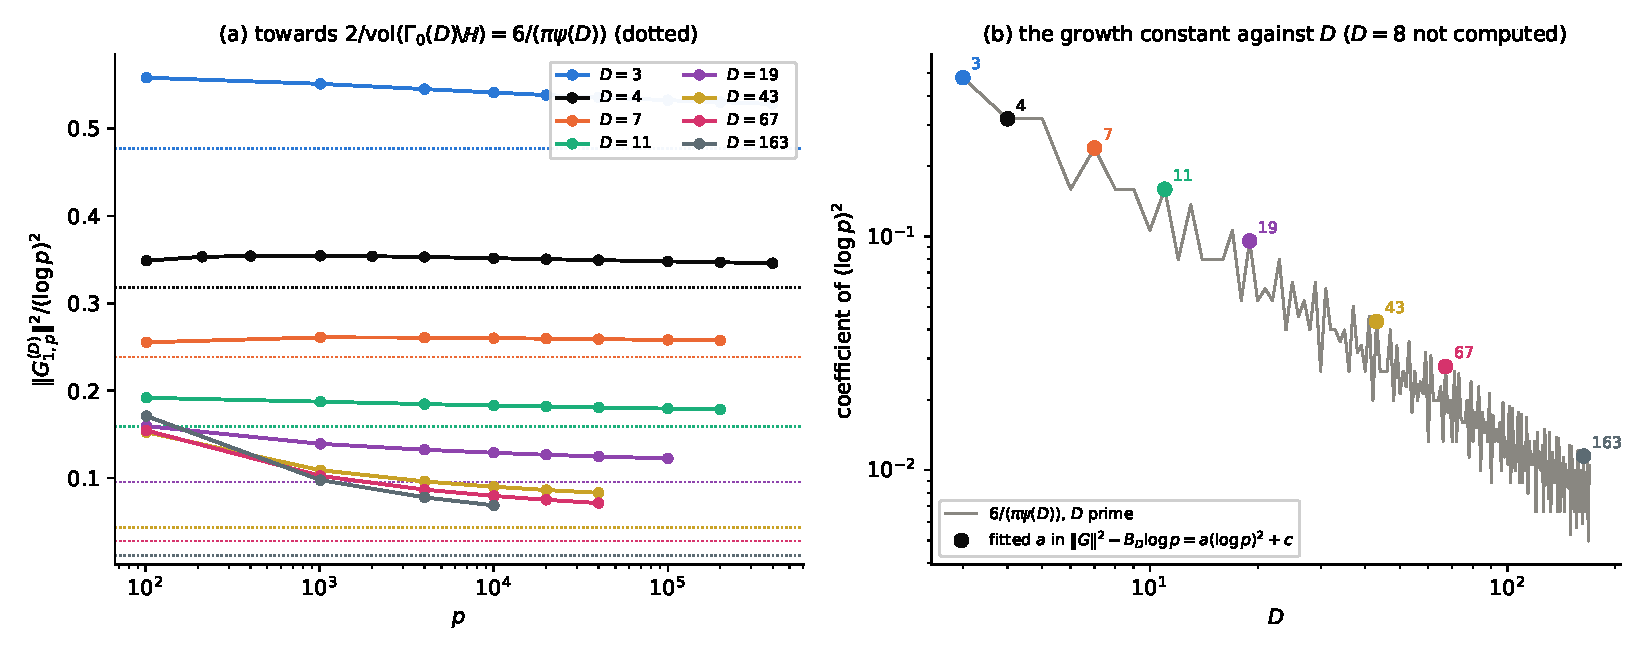
\includegraphics[width=\textwidth]{heegner_volume_scaling.pdf}
\caption{(a) $\|G^{(D)}_{1,p}\|^2/(\log p)^2$ against $p$ for $D=4$ (Table~\ref{tab:anatomy}) and the seven odd discriminants (Table~\ref{tab:oddnorm}), with the limits $2/\vol(\Gamma_0(D)\backslash\HH)=6/(\pi\psi(D))$ dotted; the approach is slow, $\frac6{\pi\psi(D)}+B_D/\log p$, and for $D\ge43$ the second term still dominates. (b) The coefficient of $(\log p)^2$ fitted with the proved $B_D$ (two parameters, $\|G\|^2-B_D\log p=a(\log p)^2+c$ over $p\ge1009$) against $D$, with the curve $6/(\pi\psi(D))$ through the primes: $0.4774$, $0.3183$, $0.2387$, $0.1591$, $0.0956$, $0.0433$, $0.0277$, $0.0115$ for $D=3,4,7,11,19,43,67,163$ against $0.4775$, $0.3183$, $0.2387$, $0.1592$, $0.0955$, $0.0434$, $0.0281$, $0.0116$; a factor $41$ between $D=3$ and $D=163$. $D=8$ has not been computed. Script \texttt{plot\_heegner\_volume\_scaling.py}; floating point.}
\label{fig:volume}
\end{figure}

\begin{figure}[htbp]
\centering
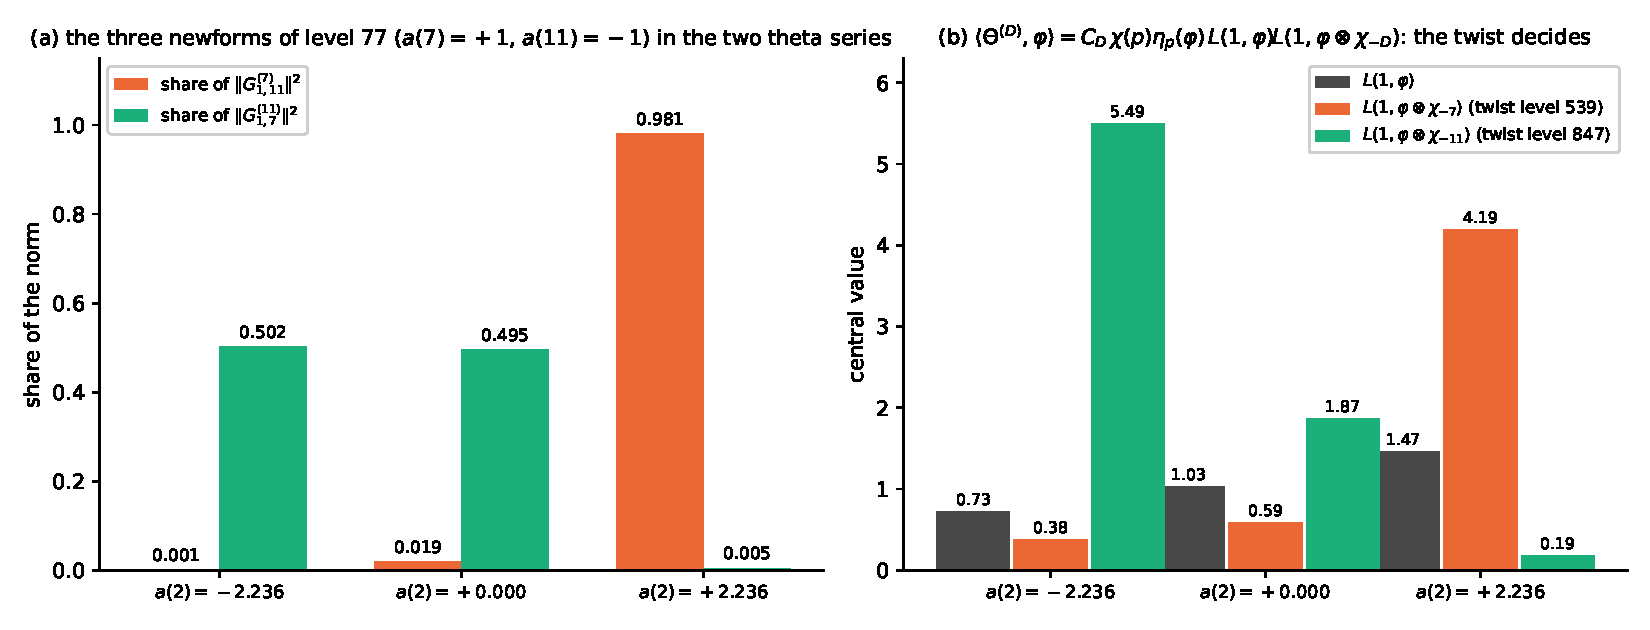
\includegraphics[width=\textwidth]{level77_duality.pdf}
\caption{The level $77$ is $7\cdot11$ in two ways. The three newforms of level $77$ with $a(7)=+1$, $a(11)=-1$ (and $a(2)=-\sqrt5,0,\sqrt5$) are exactly the support of both $G^{(7)}_{1,11}$ ($\chi_{-7}(11)=+1$: $a(7)=\chi_{-7}(11)$, $a(11)=-\chi_{-7}(11)$) and $G^{(11)}_{1,7}$ ($\chi_{-11}(7)=-1$: $a(11)=\chi_{-11}(7)$, $a(7)=-\chi_{-11}(7)$). (a) Their shares of the two norms, $0.001,0.019,0.981$ against $0.502,0.495,0.005$. (b) The central values that decide them through Theorem~\ref{thm:RS}: the same $L(1,\varphi)$, but the twists by $\chi_{-7}$ (level $539$) and by $\chi_{-11}$ (level $847$) favour opposite forms. Script \texttt{plot\_level77\_duality.py}; floating point.}
\label{fig:level77}
\end{figure}

\emph{Four different quantities.} Table~\ref{tab:oddnorm} and Theorem~\ref{thm:closedBD} involve (a) the proved constant $B_D$; (b) the exact Parseval formula, truncated at $k\le3Dp$ and $j\le8$; (c) the slope of a linear fit of $\|G\|^2-\frac6{\pi(D+1)}(\log p)^2$ over the computed primes; (d) the local slope between two consecutive primes. Only (a) is a theorem; (c) and (d) estimate it with an error that comes from the $O(1)$ term of the asymptotic formula, which is not a single constant: it depends on $p$ through $\chi_{-D}(p)$ (the densities $\beta_p$, $\beta_D$ of Theorem~\ref{thm:siegel} and the support of Theorem~\ref{thm:support}), so that the local slope between two primes with different $\chi_{-D}(p)$ carries the difference of two constants divided by $\log(p_2/p_1)$. The data show exactly this. For $D=67$ the primes $1009,4001,10007,20011,40009$ have $\chi_{-67}(p)=+,-,+,-,+$, and the local slopes alternate, $0.349$, $0.364$, $0.352$, $0.365$, around $B_{67}=0.3632$. For $D=163$ the range is the shortest ($p\le10007$, since $K=3Dp$ is limited to $8\cdot10^6$ by memory): the pair $1009,4001$ with equal $\chi_{-163}(p)=-1$ gives $0.3229$ against $B_{163}=0.3216$, and the last pair $4001,10007$, where $\chi$ changes sign, gives $0.3128$; this is the $0.009$ of Theorem~\ref{thm:closedBD}'s table, and it is the same effect, not a discrepancy with the theorem. For $D=43$ the pair $10007,20011$ with equal $\chi=+1$ gives $0.3628$ against $0.3637$. Likewise the three-parameter fits of the leading coefficient are unreliable for $D\ge43$ over these ranges ($0.045$, $0.030$, $0.0073$ against $0.0434$, $0.0281$, $0.0116$), because $B_D\log p$ is larger than $\frac6{\pi(D+1)}(\log p)^2$ there, while the two-parameter fits with $B_D$ fixed (Figure~\ref{fig:volume}) give $0.0433$, $0.0277$, $0.0115$. A run to $p=10^5$ for $D=163$ would need $K=5\cdot10^7$; we have not done it.

\emph{Truncation and rounding.} In Table~\ref{tab:oddnorm} the sums over $k$ stop at $K=3Dp$, where the smallest weight, at the cusp of width $Dp$, is $e^{-4\pi K/(Dp)}=e^{-12\pi}=4\cdot10^{-17}$; since $|a(k)|\le T(k)+M(k)\ll_\e k^{1+\e}/p$, the omitted tail $\sum_{k>K}|a(k)|^2k^{-1}e^{-4\pi k/(Dp)}$ is $\ll_\e D^2K^{2\e}e^{-12\pi}$, below $10^{-12}$ for every entry. The correlation terms with $j\ge9$ are bounded by $|\Psi_j(c)|\le e^{-\sqrt3c/2}\le e^{-9\sqrt3\pi}$, below $10^{-21}$ times the height-$1$ sum. The functions $\Psi_j$ are computed by $240$-point Gauss--Legendre quadrature in $x$ (the integrand is analytic on $[-\frac12,\frac12]$) and cubic splines on a geometric grid of $8000$ points in $c\in[10^{-9},70]$; against adaptive quadrature at $360$ random $(j,c)$ the splines are accurate to $2.5\cdot10^{-13}$ absolutely and to $10^{-9}$ relatively wherever $|\Psi_j|>10^{-6}$. The closed forms use $E_1$ from \texttt{scipy} ($10^{-15}$), $200$-point Gauss--Legendre quadrature for the $x$-integrals of $b_4^{(D)}$, adaptive quadrature ($10^{-10}$) for $I_j$, and $\beta\le4D+40$, where $E_1(4\pi\beta/D)<e^{-16\pi}$. The sums over $k$ have up to $8\cdot10^6$ non-negative terms in double precision (relative rounding below $10^{-12}$). So the entries of Table~\ref{tab:oddnorm} are correct to the digits shown, and the comparison with $B_D$ is limited by the $O(1)$ term, not by the computation.

The two curiosities of the data. At the level $77$ the same three newforms carry $G^{(7)}_{1,11}$ and $G^{(11)}_{1,7}$ with shares $(0.001,0.019,0.981)$ and $(0.502,0.495,0.005)$ (Figure~\ref{fig:level77}): the support conditions of Theorem~\ref{thm:support} coincide for the two pairs $(D,p)$, and the two twisted central values distribute the norm in opposite ways. And at $D=163$ the term $B_D\log p$ with $B_{163}=0.3216$ (Theorem~\ref{thm:closedBD}; $0.171$ of it is the tail $b_3^{(163)}$) exceeds the leading term $0.0116(\log p)^2$ for $\log p<27.6$, i.e.\ $p<10^{12}$: the suppression of the norm by the factor $41$ is, in the range of any computation, a suppression of $(\log p)^2$ only, and at $p\le10^4$ the norms of the seven odd discriminants are all between $3$ and $46$.

\section{Sieve limits and the Eisenstein dispersion form}\label{sec:eis}

\subsection{Does a large discriminant help the sieve?}\label{subsec:sieve}
For the sequence $r_D(n)r_D(N-n)$, the norm $\|G^{(D)}_{m,m'}\|^2\sim\frac6{\pi\psi(D)}(\log mm')^2$ enters the remainder through the uniform bound $|a_G(N)|\ll N^{1/2+\e}\|G\|$ (Part~I, Theorem~2.3, whose proof is independent of $D$), and it decreases like $1/D$. This does not help. The main term decreases as well: the mean value of $r_D$ is $w_DL(1,\chi_{-D})=2\pi/\sqrt D$, so $X_N=\sum_nr_D(n)r_D(N-n)\asymp\frac{4\pi^2}DN\mathfrak S_D(N)$ is of size $N/D$, while the remainder for one pair $(d,e)$ of sieve moduli is $\ll N^{1/2+\e}(\log de)/\sqrt{\psi(D)}$; the ratio remainder/main is $\asymp\sqrt D\,N^{-1/2}\log de$ for prime $D$, larger by $\sqrt D$, not smaller. And the level of distribution is an exponent while $D$ is fixed: the proof of the level $1/2$ (Part~I, Theorem~3.2) loses only constants and $N^\e$ in $D$, so the level is $1/2$ for every $D$, and the sieve dimension is $2$ for every $D$, since $\sum_{p\le z}\omega_D(p)/p=2\log\log z+O(1)$ with $\omega_D(p)=2(1+\chi_{-D}(p))$ on average. What a large discriminant changes is the constant in the final count, $\asymp N/(D(\log N)^2)$, and, for the odd $D$, the shape of the fundamental domain, which simplifies the norm and has no bearing on the dispersion problem.

\subsection{The circle modulo \texorpdfstring{$c$}{c} for the Eisenstein integers}
\begin{lemma}\label{lem:circle3}
Let $(c,3)=1$, $c$ odd or even, $(a,c)=1$, $h\in\Z^2$, $|h|_3^2=h_1^2-h_1h_2+h_2^2$, $c'^{*}$ the product of the primes dividing $c'$ to an odd power, and $\chi=\chi_{-3}$ ($\chi(2)=-1$). Then
\[
F_c(a;h):=\sum_{\substack{x,y\bmod c\\ N_3(x,y)\equiv a\ (c)}}e\Bigl(\frac{h_1x+h_2y}c\Bigr)=\sum_{g\mid(c,h_1,h_2)}g\,\chi\Bigl(\Bigl(\frac cg\Bigr)^{*}\Bigr)S\Bigl(a,\ \overline3\,\Bigl|\frac hg\Bigr|_3^2;\ \frac cg\Bigr).
\]
\end{lemma}
\begin{proof}
Write $N_3(x)=\frac12x^{\mathsf T}Ax$ for $x=(x,y)$ with the Gram matrix $A=\left(\begin{smallmatrix}2&1\\1&2\end{smallmatrix}\right)$, $\det A=3$, and put $G_A(t;c)=\sum_{x\bmod c}e(tN_3(x)/c)$ for $(t,c)=1$. Three steps; the first two are the Gauss sums of the hexagonal lattice, for which see also \cite[Chapter~1]{BEW} and \cite[Section~3.5]{IK}.

\emph{Step 1: $G_A(t;c)=\chi(c)\,c$ for every $c$ prime to $3$ and every $t$ prime to $c$.} For $(c_1,c_2)=1$ write $x=c_2x_1+c_1x_2$; then $N_3(x)\equiv c_2^2N_3(x_1)+c_1^2N_3(x_2)\pmod{c_1c_2}$, the cross term $c_1c_2\,x_1^{\mathsf T}Ax_2$ being divisible by $c_1c_2$, so $G_A(t;c_1c_2)=G_A(tc_2;c_1)\,G_A(tc_1;c_2)$ and it suffices to treat $c=\ell^\nu$. For $\nu\ge2$ write $x=x_0+\ell^{\nu-1}x_1$ with $x_0$ modulo $\ell^{\nu-1}$ and $x_1$ modulo $\ell$: $N_3(x)\equiv N_3(x_0)+\ell^{\nu-1}x_0^{\mathsf T}Ax_1\pmod{\ell^\nu}$, the sum over $x_1$ is $\ell^2[Ax_0\equiv0\ (\ell)]=\ell^2[x_0\equiv0\ (\ell)]$ because $A$ is invertible modulo $\ell\ne3$, and with $x_0=\ell x_0'$ this gives $G_A(t;\ell^\nu)=\ell^2G_A(t;\ell^{\nu-2})$. Hence $G_A(t;\ell^\nu)=\ell^\nu$ for even $\nu$ and $\ell^{\nu-1}G_A(t;\ell)$ for odd $\nu$. For $\nu=1$ and $\ell\ne2$, $4N_3=(2x+y)^2+3y^2$ and the substitution $(2x+y,y)\mapsto(x,y)$ (a bijection modulo $\ell$) give $G_A(t;\ell)=G(\bar4t;\ell)G(3\bar4t;\ell)$ with $G(a;\ell)=\sum_xe(ax^2/\ell)=\bigl(\frac a\ell\bigr)\varepsilon_\ell\sqrt\ell$, $\varepsilon_\ell^2=\bigl(\frac{-1}\ell\bigr)$, so $G_A(t;\ell)=\bigl(\frac3\ell\bigr)\bigl(\frac{-1}\ell\bigr)\ell=\bigl(\frac{-3}\ell\bigr)\ell=\chi(\ell)\ell$; and directly $G_A(t;2)=1-1-1-1=-2=\chi(2)\cdot2$. So $G_A(t;\ell^\nu)=\chi(\ell)^\nu\ell^\nu$ in every case, independently of $t$, and the multiplicativity gives $G_A(t;c)=\chi(c)c$; this equals $\chi(c^{*})c$ because $\chi(\ell)^2=1$ for $\ell\ne3$.

\emph{Step 2: completing the square.} For $(t,c)=1$ and $h\in\Z^2$ the vector $v=\bar t\,A^{-1}h$ is defined modulo $c$, since $A^{-1}=\frac13\left(\begin{smallmatrix}2&-1\\-1&2\end{smallmatrix}\right)$ and $3$ is invertible modulo $c$; and $tN_3(x+v)=tN_3(x)+t\,x^{\mathsf T}Av+tN_3(v)=tN_3(x)+h\cdot x+\bar t\,\tfrac12h^{\mathsf T}A^{-1}h$, where $\frac12h^{\mathsf T}A^{-1}h=\frac13(h_1^2-h_1h_2+h_2^2)=\frac13|h|_3^2$. Both sides are polynomials with integer coefficients in $x$ and $v$ ($N_3(x)=x^2+xy+y^2$), so no division by $2$ occurs, and $\sum_{x\bmod c}e\bigl((tN_3(x)+h\cdot x)/c\bigr)=e(-\bar t\,\bar3\,|h|_3^2/c)\,G_A(t;c)$.

\emph{Step 3: the sum over $t$.} $F_c(a;h)=\frac1c\sum_{t\bmod c}e(-ta/c)\sum_{x\bmod c}e((tN_3(x)+h\cdot x)/c)$. For $(t,c)=g$ write $t=gt'$, $c=gc'$ and $x=x_0+c'x_1$ with $x_0$ modulo $c'$, $x_1$ modulo $g$: $tN_3(x)/c\equiv t'N_3(x_0)/c'$ and $h\cdot x/c=h\cdot x_0/c+h\cdot x_1/g$ modulo $1$, so the sum over $x_1$ is $g^2[g\mid h]$, and for $g\mid h$ the sum over $x_0$ is $\sum_{x_0\bmod c'}e((t'N_3(x_0)+(h/g)\cdot x_0)/c')=e(-\bar t'\,\bar3\,|h/g|_3^2/c')\,\chi(c')c'$ by Steps~1 and 2. Collecting the $t'$ prime to $c'$,
\[
F_c(a;h)=\sum_{g\mid(c,h)}\frac{g^2c'}{c}\,\chi(c')\sum_{t'\bmod c'}^{*}e\Bigl(\frac{-t'a-\bar t'\,\bar3\,|h/g|_3^2}{c'}\Bigr)=\sum_{g\mid(c,h)}g\,\chi\Bigl(\frac cg\Bigr)S\Bigl(a,\ \bar3\Bigl|\frac hg\Bigr|_3^2;\ \frac cg\Bigr),
\]
by $S(-m,-n;c')=S(m,n;c')$ ($t'\mapsto-t'$); for $c'=1$ both $G_A$ and $S$ are $1$. The script \texttt{eisenstein\_circle\_check.py} verifies the identity for all $a$, $h$ and all $c\le40$ prime to $3$, odd and even ($285\,902$ cases).
\end{proof}

\subsection{The dispersion form}
Let $m,m'$ be coprime square-free integers prime to $3N$. Since the ideal $(\sqrt{-3})$ is principal of norm $3$, $r_3(3\beta')=r_3(\beta')$, and the terms of $T(m,m';N)$ with $3\mid\beta$ are $T(m,3m';N)$: with $T^\flat(m,m';N)=\sum_{3\nmid\beta}r_3(\alpha)r_3(\beta)$,
\[
a_{G_{m,m'}}(N)-a_{G_{m,3m'}}(N)=T^\flat(m,m';N)-M^\flat(m,m';N),
\]
the analogue of $a_G(N)-a_G(N/2)=T^{\mathrm{odd}}-M^{\mathrm{odd}}$ of Part~III. In $T^\flat$, $r_3(\beta)\ne0$ forces $\beta\equiv1\pmod3$, so $\chi(\beta/k)=\chi(k)$ and $r_3(\beta)=12\sum_{k\mid\beta,\,k<\sqrt\beta}\chi(k)+6\chi(\sqrt\beta)[\beta=\square]$, the divisors $k$ being prime to $3$ and to $m$ but possibly even. Hence
\begin{gather*}
T^\flat(m,m';N)=12\sum_{\substack{k<\sqrt{N/m'}\\ 3\nmid k}}\chi(k)\,\mathcal N_k+6\sum_j\chi(j)\,r_3^\flat\Bigl(\frac{N-m'j^2}m\Bigr),\\
\mathcal N_k=\#\Bigl\{(x,y):\ N_3(x,y)\equiv N\bar m\ (m'k),\ mN_3(x,y)\not\equiv N\ (3),\ 0<N_3(x,y)<Y_k\Bigr\},
\end{gather*}
$Y_k=(N-m'k^2)/m$. The condition modulo $3$ is the analogue of the parity condition $x+y$ odd of Part~III: Poisson summation on the classes modulo $3c$, $c=m'k$, gives
\[
\mathcal N_k=\frac{Y_k}{(3c)^2}\sum_{h\in\Z^2}\hat w\Bigl(\frac{h\sqrt{Y_k}}{3c}\Bigr)\,\epsilon_3(h)\,F_c(N\bar m;\ \bar3h),
\]
where $\bar3h$ is the Chinese-remainder twist and $\epsilon_3(h)$ the Fourier transform of the admissible classes modulo $3$: as $N_3(x,y)\equiv(x-y)^2\pmod3$, the condition is $x\equiv y$ if $N\bar m\equiv1$, $x\not\equiv y$ if $N\bar m\equiv0$, and empty if $N\bar m\equiv2\pmod3$, so that $\epsilon_3(h)=3[h_1+h_2\equiv0\ (3)]$, $9[h\equiv0\ (3)]-3[h_1+h_2\equiv0\ (3)]$, $9$, respectively. Since $|h|_3^2\equiv(h_1+h_2)^2\pmod3$, the condition $h_1+h_2\equiv0\pmod3$ is $3\mid|h|_3^2$: exactly the condition $h_1\equiv h_2\pmod2$, i.e.\ $2\mid|h|^2$, of Part~III, with the ramified prime of the field in the role of $2$. By Lemma~\ref{lem:circle3} applied to the vector $\bar3h$, whose norm is $|\bar3h|_3^2\equiv\bar9|h|_3^2\pmod c$, the leading term $g=1$ of $F_c(N\bar m;\bar3h)$ is $\chi((m'k)^{*})S(N\bar m,\bar3\cdot\bar9|h|_3^2;m'k)=\chi((m'k)^{*})S(N\bar m,\overline{27}|h|_3^2;m'k)=\chi((m'k)^{*})S(\overline{27m}N,|h|_3^2;m'k)$, the last step because a Kloosterman sum depends on its two arguments only through their product, here $N\bar m\cdot\overline{27}|h|_3^2=\overline{27m}N|h|_3^2$ modulo $m'k$ (Section~\ref{sec:intro}.3; checked numerically in \texttt{kloosterman\_argument\_audit.py}); and $\chi(k)\chi((m'k)^{*})=\chi(m')$ for square-free $m'$.

\begin{proposition}\label{prop:eisdisp}
The leading term ($g=1$) of $a_{G_{m,m'}}(N)-a_{G_{m,3m'}}(N)$ is
\[
12\,\chi(m')\sum_{\substack{k<\sqrt{N/m'}\\ 3\nmid k}}\frac{Y_k}{(3m'k)^2}\sum_{h\ne0}\hat w\Bigl(\frac{h\sqrt{Y_k}}{3m'k}\Bigr)\,\epsilon_3(h)\,S\bigl(\overline{27m}\,N,\ |h|_3^2;\ m'k\bigr),
\]
and the remainder sum of the sieve at the level $N^\theta$ has as its leading term the trilinear form $\sum_{m'}\Lambda'_{m'}\sum_{c\equiv0\,(m')}\sum_m\Lambda_m\sum_jb_{m,j}(c)S(\overline{27m}N,j;c)$ over the moduli $c=m'k$ prime to $3$, odd or even, with $j=|h|_3^2\ll mm'$ a norm from $\Z[\zeta_3]$, whose $m$-th piece is, by the Chinese remainder theorem, the bilinear form in the two moduli
\[
\mathfrak B^{(3)}_m=\sum_{m'}\Lambda'_{m'}\sum_{k\le K}\sum_hw_{k,m'}(h)\,S\bigl(\overline{27m}N\bar k,\ |h|_3^2\bar k;\ m'\bigr)\,S\bigl(\overline{27m}N\overline{m'},\ |h|_3^2\overline{m'};\ k\bigr).
\]
\end{proposition}

\emph{What is an identity and what is a bound.} Behind Proposition~\ref{prop:eisdisp} is the exact decomposition, as in Part~III, Proposition~3.2,
\[
a_{G_{m,m'}}(N)-a_{G_{m,3m'}}(N)=R_1+R_{g>1}+\Sigma_\square+\Sigma_\partial ,
\]
where $R_1$ is the displayed leading term (the terms $g=1$, $h\ne0$ of Lemma~\ref{lem:circle3}; the terms $h=0$, summed over $k$, are the Siegel main term $M^\flat$), $R_{g>1}$ collects the terms $g\mid(m'k,h)$ with $g>1$, sums of the same shape with the modulus $m'k/g$ and the dual variable $h/g$, $\Sigma_\square=6\sum_j\chi(j)r_3^\flat((N-m'j^2)/m)\ll N^{1/2+\e}m'^{-1/2}$ is the ternary term, and $\Sigma_\partial$ the error of the smooth cutoff at $Y_k$. This identity, Lemma~\ref{lem:circle3} and the shape of the bilinear form are what is proved here. The bounds for $R_1$ that are asserted are exactly those of Part~III, which only open the Kloosterman sums or use their Weil mean square: the Weil bound $|S(a,|h|_3^2;c)|\le d(c)c^{1/2}(|h|_3^2,c)^{1/2}$ gives the level $1/4$, the theta-function bound (Part~I, Theorem~2.3, whose proof applies to $\theta_3$ unchanged) the level $1/2$, and the Cauchy--Schwarz arrangements (A1), (A2) and the Poisson step in $h$ of Part~III, Section~4, transfer verbatim because they depend only on the lengths of the variables ($|h|\ll m'k\sqrt{m/N}$, $H\le\sqrt{mm'}$) and on $\sum_h|S|^2$. No bound beyond the level $1/2$ is proved or claimed, for $R_1$ or for the whole remainder, and $R_{g>1}$, $\Sigma_\square$, $\Sigma_\partial$ are not estimated here, exactly as in Part~III, Remark~3.3(iv).

\emph{Comparison with the Gaussian case.} Nothing in the structure changes. (i) The fixed argument is the single integer $N$, carried by a unit ($\overline{27m}$ in place of $\overline{16m}$) modulo the modulus, so the obstacle of Part~III, Section~3.4, the absence of an average over it and the inapplicability of the Kuznetsov formula and of the bounds of \cite{DI,Drappeau}, is the same. (ii) The sizes are the same: $|h|\ll m'k\sqrt{m/N}$, the $h$-box has side $H\le\sqrt{mm'}$, below $\sqrt q$ for every modulus $q=[c_1,c_2]$ of a Poisson step, and the Cauchy--Schwarz arrangements (A1), (A2) of Part~III, Section~4 give the same diagonals ($E^{1/4}N^{3/4}$ and $\sqrt{EN}$); there is no tighter grouping, because the groupings depend only on the lengths of the variables and on the Weil mean square of Kloosterman sums over the dual lattice, which is the same for the hexagonal lattice. (iii) The moduli $m'k$ range over all $k$ prime to $3$, even $k$ included: more moduli, no gain. (iv) The $2$-adic ``impurity'' of Part~III has moved to $3$: the condition $3\nmid\beta$ produces $\epsilon_3(h)$ and $3\mid|h|_3^2$, as $2\nmid\beta$ produced $h_1\equiv h_2\pmod2$. This is not an accident: the ramified prime is where the ideal of norm $\ell$ is principal, and removing it from the divisor sum of $r_D(\beta)$ is what makes the divisors $k<\sqrt\beta$ pair with $\beta/k$ under $\chi$. The clean level $Dp$ matters for the holomorphic side (Section~\ref{sec:heegner}), not for the dispersion form; a level beyond $1/2$ needs the bilinear saving over $(m',k)$ of Part~III, Section~4.5, in the Eisenstein setting as in the Gaussian one.

\section{Outlook}\label{sec:outlook}
The problem of Parts I--IV, $N=n+(N-n)$ with both summands norms from an imaginary quadratic field of class number one and few prime factors, is a binary additive problem of the Goldbach type with two sparse sequences, and it shares with Goldbach's problem the shape of its obstacles: a level of distribution $1/2$ obtained from the modular side (here from a theta series, there from the Bombieri--Vinogradov theorem), a sieve whose dimension (here $2$) fixes the attainable pair $(k,k')$ at that level, and a remainder beyond $1/2$ that is a bilinear form in Kloosterman sums with one argument fixed. What the present part adds to this picture is structural. The spectral support of the theta series is governed by the Atkin--Lehner signs at the ramified prime and at $p$ (Theorem~\ref{thm:support}): the remainder sees only the newforms whose root number is $+1$ and whose signs match $\chi_{-D}(p)$, so the parity of the root number, which decides the vanishing of $L(1,\varphi)$, enters the sieve remainder at the level of individual forms; the Rankin--Selberg formula (Theorem~\ref{thm:RS}) writes the remainder as a sum of products of two central values, a twist by $\chi_{-D}$ against the trivial one, so that the automorphic lift to $\mathrm{GL}_2$ of the two quadratic fields (the one of the discriminant and the one of the twist) is where the arithmetic of $N$ is encoded; and the norm, which measures the size of the remainder on average, is the reciprocal volume of $X_0(D)$ (Theorem~\ref{thm:B}(v)), the modular curve of the discriminant, which is rational for the four small discriminants $D\in\{3,4,7,8\}$ and has genus $1,1,3,5,13$ for $D=11,19,43,67,163$; the second coefficient $B_D$ (Theorems~\ref{thm:closedB} and \ref{thm:closedBD}) has, for all eight discriminants treated, the same five pieces, the free part, the arcs, the tail of exponential integrals at the two wide cusps, its arcs, and the correlations, so that a uniform formula for $B_D$ over imaginary quadratic fields, with the class group entering through the theta series of the classes, seems within reach, and would be the natural continuation. We do not claim that any of this moves the Goldbach problem; the honest content is that the two problems have the same anatomy, and that in the theta-series setting every piece of that anatomy (main term, support, central values, norm) has been made explicit. The question that remains, here as there, is the bilinear form of Part~III, Section~4.5.

\section*{Data and code}
{\raggedright
The scripts \texttt{subleading\_log\_anatomy.py} and \texttt{closed\_form\_B.py} (Section~\ref{sec:scallop}; they import the tables and the Siegel main term of Part~II), \texttt{heegner\_theta\_unified.py} and \texttt{heegner\_closed\_form\_B.py} (Sections~\ref{sec:heegner}--\ref{sec:num}), \texttt{eisenstein\_circle\_check.py} (Lemma~\ref{lem:circle3}), \texttt{kloosterman\_argument\_audit.py} (Sections~\ref{sec:intro}.3 and \ref{sec:eis}) and the plotting scripts \texttt{plot\_scalloped\_anatomy.py}, \texttt{plot\_heegner\_volume\_scaling.py}, \texttt{plot\_level77\_duality.py}, with their outputs in \texttt{results/} and the working notes in \texttt{notes/}, are in the repository \url{https://github.com/Ruqing1963/two-squares-part4}. All computations are in floating point and are evidence, not proof; the theorems do not depend on them.
\par}

\begin{thebibliography}{99}\raggedright
\bibitem{AL} A.~O.~L. Atkin and J. Lehner, Hecke operators on $\Gamma_0(m)$, Math. Ann. 185 (1970), 134--160.
\bibitem{BEW} B.~C. Berndt, R.~J. Evans and K.~S. Williams, Gauss and Jacobi Sums, Wiley, New York, 1998.
\bibitem{ChenI} R. Chen, Sums of two squares with few prime factors via theta series of quaternary forms, preprint (2026), doi:10.5281/zenodo.23826176.
\bibitem{ChenII} R. Chen, Sums of two squares with few prime factors, II: the mean square of the cuspidal error of $\theta^2(mz)\theta^2(m'z)$, almost all $N$, and the size of the Petersson norm, preprint (2026), doi:10.5281/zenodo.23826297 (corrected version in the repository).
\bibitem{ChenIII} R. Chen, Sums of two squares with few prime factors, III: the dispersion obstacle, sieve barriers at the level $1/2$, and short-interval mean squares, preprint (2026), doi:10.5281/zenodo.23826860 (corrected version in the repository).
\bibitem{DI} J.-M. Deshouillers and H. Iwaniec, Kloosterman sums and Fourier coefficients of cusp forms, Invent. Math. 70 (1982), 219--288.
\bibitem{DS} F. Diamond and J. Shurman, A First Course in Modular Forms, Springer, 2005.
\bibitem{Drappeau} S. Drappeau, Sums of Kloosterman sums in arithmetic progressions, and the error term in the dispersion method, Proc. London Math. Soc. 114 (2017), 684--732.
\bibitem{IK} H. Iwaniec and E. Kowalski, Analytic Number Theory, AMS Colloquium Publications 53, 2004.
\bibitem{Kitaoka} Y. Kitaoka, Arithmetic of Quadratic Forms, Cambridge Tracts in Mathematics 106, Cambridge University Press, 1993.
\bibitem{Martin} K. Martin, Refined dimensions of cusp forms, and equidistribution and bias of signs, J. Number Theory 188 (2018), 1--17; arXiv:1609.05386.
\bibitem{Siegel} C.~L. Siegel, \"Uber die analytische Theorie der quadratischen Formen, Ann. of Math. 36 (1935), 527--606.
\bibitem{Stark} H.~M. Stark, A complete determination of the complex quadratic fields of class-number one, Michigan Math. J. 14 (1967), 1--27.
\bibitem{Waibel} F. Waibel, Uniform bounds for norms of theta series and arithmetic applications, Math. Proc. Cambridge Philos. Soc. 173 (2022), 669--691; arXiv:2012.04311 (equation numbers refer to the arXiv version).
\bibitem{Yamauchi} M. Yamauchi, On the traces of Hecke operators for a normalizer of $\Gamma_0(N)$, J. Math. Kyoto Univ. 13 (1973), 403--411.
\end{thebibliography}
\end{document}
